\documentclass[10pt,a4paper,twoside,titlepage,twocolumn]{article}
\usepackage[utf8]{inputenc}
\usepackage[T1]{fontenc}
\usepackage[ngerman]{babel,varioref}
\usepackage[left=0.7cm,right=0.7cm,top=0.7cm,bottom=0.7cm,includeheadfoot]{geometry}

\usepackage{amsmath}
\usepackage{amssymb}
\usepackage{graphicx}
\usepackage{xcolor}
\usepackage{siunitx}



\begin{document}
    \graphicspath{ {./Images/} }


\definecolor{formulablue}{RGB}{219,219,255}
\newcommand{\formula}[1]{\colorbox{formulablue}{#1}}

\newcommand{\unitText}[3]{\noindent\textit{#1} : #2 [#3]}

\definecolor{refrot}{RGB}{183,28,42}
\newcommand{\refskript}[1]{\textcolor{refrot}{Skript S.#1}}



% \titlespacing*{\section}{0pt}{12pt}{0pt}
% \titlespacing*{\subsection}{0pt}{0pt}{0pt}
% \titlespacing*{\subsubsection}{0pt}{0pt}{0pt}


\title{\vspace{50mm}AdvDeLearn \\ [1ex] \large Summary}
\author{Lukas Schöpf}
% \titlepic{\vspace{50mm}\includegraphics[width=0.25\textwidth]{Elvis}}


% Code format
% Define the Gruvbox light colors
\definecolor{gruvbox_bg}{HTML}{fbf1c7}
\definecolor{gruvbox_fg}{HTML}{3c3836}
\definecolor{gruvbox_yellow}{HTML}{d79921}
\definecolor{gruvbox_red}{HTML}{cc241d}
\definecolor{gruvbox_green}{HTML}{98971a}
\definecolor{gruvbox_blue}{HTML}{458588}
\definecolor{gruvbox_purple}{HTML}{b16286}
\definecolor{gruvbox_aqua}{HTML}{689d6a}
\definecolor{gruvbox_orange}{HTML}{d65d0e}


% \lstdefinestyle{cppstyle}{
% 	language=C++,
% 	basicstyle=\ttfamily\footnotesize,
% 	numbers=left,
% 	numberstyle=\tiny,
% 	numbersep=5pt,
% 	tabsize=4,
% 	showspaces=false,
% 	showstringspaces=false,
% 	frame=single,
% 	rulecolor=\color{gruvbox_fg},
% 	backgroundcolor=\color{white},
% 	keywordstyle=\color{gruvbox_orange},
% 	commentstyle=\color{gruvbox_aqua},
% 	stringstyle=\color{gruvbox_green},
% 	identifierstyle=\color{gruvbox_fg},
% 	emphstyle=\color{gruvbox_red},
% 	emph={int, double, string, cout, TimerHandle_t, BaseType_t, timerPWMPeripheral_t, SemaphoreHandle_t, TaskHandle_t, QueueHandle_t},
% 	xleftmargin=5mm,
% 	xrightmargin=\parindent
% }

	\maketitle
	\setlength\parindent{0pt}

	% Uncomment these lines if you want to include the respective sections
	\section{Deep Learning Recap}

\subsection{Neural Network Types}
\subsubsection{Multi-Layer Perceptron (MLP)}
\begin{itemize}
    \item Input: \( n \)-dimensional, Output: \( m \)-dimensional.
    \item Fully connected hidden layers.
    \item Applications: Classification, regression, feature transformation, and dimensionality reduction.
\end{itemize}
Base equation / shallow network:
\[
f(x) = \sum_{i = 1}^{N} a_i \sigma(\mathbf{w}_i\cdot\mathbf{x} + b_i)
\]
For deep network:
\[
    y = f_3(f_2(f_1(x)))
\]

\subsubsection{Convolutional Neural Networks (CNNs)}
\begin{itemize}
    \item Feature extraction through convolutional layers.
    \item Supports multi-channel inputs (e.g., RGB images).
    \item Applications: Image processing, signal analysis, time-series data, 3D datasets like MRI.
\end{itemize}
Properties:
\begin{itemize}
    \item Weights(parameters) are shared
    \item Connections are sparse
    \item Each node in a layer has a receptive field
\end{itemize}
For multi-channel inputs, a diffrent kernel is applied for each channel.
The resulting channels are summed:
\[
C_{out,j} = b_j + \sum_{k=0}^{C_{in}-1} w \star f(x,y)
\]

Good practiec is to replace large filters with multiple smaller.

\subsection{Key Architectural Patterns}
\subsubsection{Reducing and Increasing Output Size}
\begin{itemize}
    \item Techniques: Strided convolutions, pooling, upsampling, and transposed convolutions.
\end{itemize}

\subsubsection{Improving Efficiency}
\begin{itemize}
    \item Bottleneck layers: Use \( 1 \times 1 \) convolutions to reduce channel dimensions.
    \item Separable filtes(for $7\times7$ use $(7\times1) \cdot (1\times7)$).
    \item Depthwise separable convolutions for sparse connectivity.
    \item Instead of one $11 \times 11$ conv. layer use 5 $3\times3$.
\end{itemize}

\subsubsection{Residual Connections}
\begin{itemize}
    \item Allow better gradient flow in deep networks.
    \item Key to ResNet architectures.
\end{itemize}

\subsubsection{Regularization}
\begin{itemize}
    \item Techniques: Dropout, \( L_2 \)-regularization.
    \item Goal: Prevent overfitting and improve generalization.
\end{itemize}

\subsection{Training Considerations}
\subsubsection{Layer/Batch normalization}
\begin{itemize}
    \item Use to normalize input to layers
    \item Accelerates training, importves generalization
\end{itemize}
\begin{equation*}
    \hat{x}^{(i)} = \frac{x^{(i)} - \mu_{\text{batch}}}{\sqrt{\sigma^2_{\text{batch}} + \epsilon}}
\end{equation*}
    
\begin{equation*}
    y^{(i)} = \gamma \hat{x}^{(i)} + \beta
\end{equation*}
\(\gamma\) and \(\beta\) are learnd from mini batches.

\subsubsection{Weight Initialization}
\begin{itemize}
    \item Xavier initialization ensures variance proportionality.
\end{itemize}

\subsubsection{Activation Functions}
\begin{itemize}
    \item Options: ReLU, Leaky ReLU, Sigmoid, Tanh, etc.
    \item ReLU variants preferred for stability.
\end{itemize}

\subsubsection{Optimizers}
\begin{itemize}
    \item Popular choices: SGD, Adam, RMSprop.
    \item Trade-offs between convergence speed and generalization.
\end{itemize}


	\section{Attention and Transformers}
\begin{figure}[ht]
    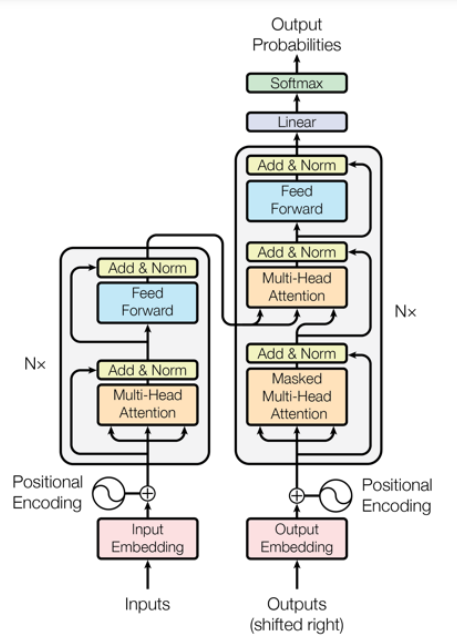
\includegraphics[width=0.6\columnwidth]{figures/AttentionTransformer/Transformer.png}
\end{figure}
\subsection{Sequence Processing}
\subsubsection{Recurrent Neural Networks (RNNs)}
\begin{itemize}
    \item Process sequences using recurrent cells with an internal state \( h \).
    \item Computation at each time step:
    \[
    h_t = \sigma(W_{hh} h_{t-1} + W_{xh} x_t + b_h)
    \]
    \item Output:
    \[
    y_t = W_{hy} h_t + b_y
    \]
    \item Common challenges: vanishing and exploding gradients.
\end{itemize}

\subsubsection{Advanced RNN Variants}
\begin{itemize}
    \item LSTMs handle long-term dependencies using gates:
    \[
    c_t = f_t \odot c_{t-1} + i_t \odot \tanh(W_c x_t + U_c h_{t-1} + b_c)
    \]
    \[
    h_t = o_t \odot \tanh(c_t)
    \]
    \item \(c_t\) long term memory
    \item \(h_t\) short term /working memory
    \item GRUs simplify LSTMs by merging the forget and input gates:
    \[
    h_t = (1 - z_t) \odot h_{t-1} + z_t \odot \tilde{h}_t
    \]
\end{itemize}
\begin{figure}
    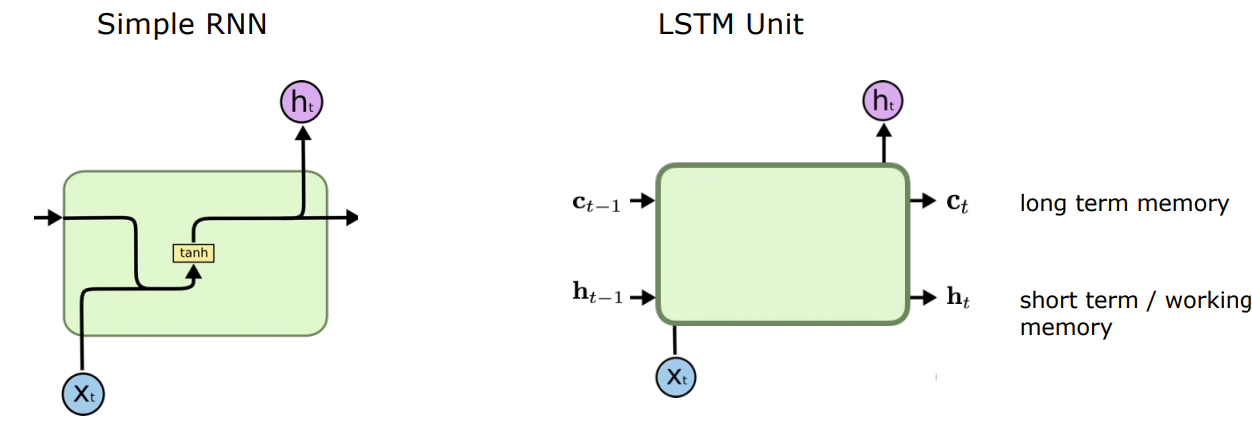
\includegraphics[width= \columnwidth]{figures/AttentionTransformer/RNNLSTM.png}
\end{figure}
\subsection{Attention Mechanism}
\subsubsection{Concept and Applications}
\begin{itemize}
    \item Attention aligns inputs with outputs for tasks like translation and image captioning.
    \item Improves handling of long sequences and offers interpretability.
\end{itemize}

\subsubsection{Attention Calculation}
\begin{itemize}
    \item Compute attention weights:
    \[
    \text{score}(q, k) = \frac{q \cdot k}{\sqrt{d_k}}
    \]
    \item Normalize weights with softmax:
    \[
    \alpha_{ij} = \frac{\exp(\text{score}(q_i, k_j))}{\sum_{j'} \exp(\text{score}(q_i, k_{j'}))}
    \]
    \item Compute the attention output as a weighted sum of values:
    \[
    \text{Attention}(Q, K, V) = \text{softmax}\left(\frac{QK^\top}{\sqrt{d_k}}\right)V
    \]
\end{itemize}

\subsection{Transformer Architecture}

\subsubsection{Encoder Architecture}
\begin{itemize}
    \item The encoder consists of \( N \) identical layers, each with:
    \begin{enumerate}
        \item Multi-head self-attention:
        \[
        \text{MultiHead}(Q, K, V) = \text{Concat}(\text{head}_1, \ldots, \text{head}_h)W^O
        \]
        where
        \[
        \text{head}_i = \text{Attention}(QW_i^Q, KW_i^K, VW_i^V)
        \]
        \item A feedforward network applied to each position:
        \[
        \text{FFN}(x) = \text{ReLU}(0, xW_1 + b_1)W_2 + b_2
        \]
        \item Residual connections and layer normalization for stability:
        \[
        \text{Output} = \text{LayerNorm}(x + \text{SubLayer}(x))
        \]
    \end{enumerate}
\end{itemize}

\subsubsection{Decoder Architecture}
\begin{itemize}
    \item The decoder mirrors the encoder but includes an additional sub-layer for cross-attention:
    \begin{enumerate}
        \item Masked multi-head self-attention:
        \[
        \text{Attention}(Q, K, V) = \text{softmax}\left(\frac{QK^\top}{\sqrt{d_k}}\right)V
        \]
        Masking prevents the decoder from seeing future tokens during training.
        \item Cross-attention, where queries come from the decoder, and keys/values come from the encoder.
        \item Feedforward network and residual connections (as in the encoder).
    \end{enumerate}
    \item A final linear layer projects the decoder's output to the vocabulary size, followed by a softmax:
    \[
    p(y_t | y_{<t}, x) = \text{softmax}(W_s h_t + b_s)
    \]
\end{itemize}

\subsubsection{Positional Encoding}
\begin{itemize}
    \item Adds sequence order information:
    \[
    PE_{\text{pos}, 2i} = \sin\left(\frac{\text{pos}}{10000^{2i/d_{\text{model}}}}\right)
    \]
    \[
    PE_{\text{pos}, 2i+1} = \cos\left(\frac{\text{pos}}{10000^{2i/d_{\text{model}}}}\right)
    \]
\end{itemize}
	\section{Vision Transformer (ViT)}
\begin{figure}[]
    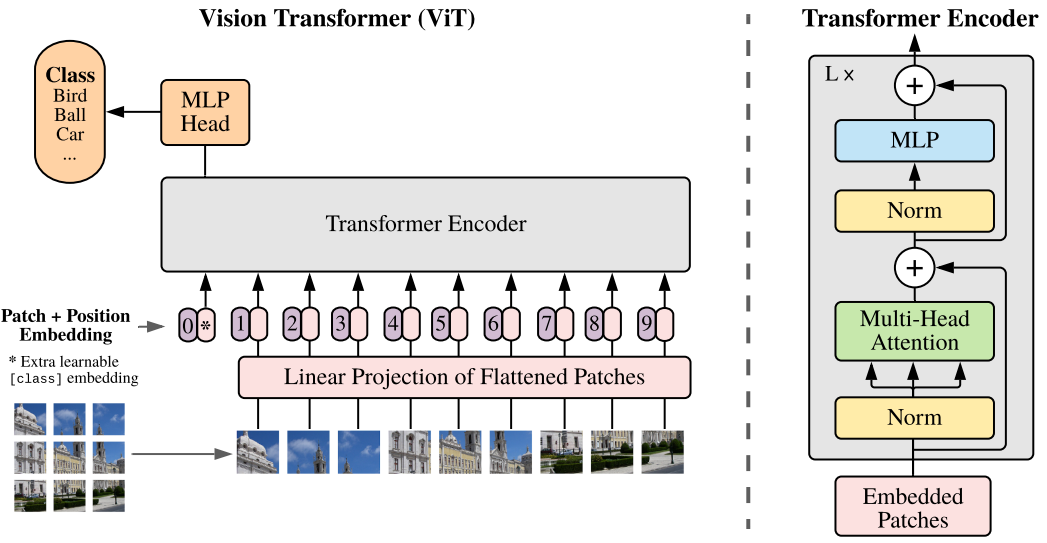
\includegraphics[width=\columnwidth]{figures/VisionTransformer/ViT.png}
\end{figure}
\begin{itemize}
    \item Extract square Images Patches
    \item Flatten Patches and project them to the embedding dimension D
    \item These embeddings are input to the Transformer
    \item Output of Transformer is fed into MLP or a singel layer
    \item Position embeddings added to input embeddings
\end{itemize}

Excellent results when pretrained on larger dataset(14M-300M)images and fine-tuned.

\subsection{Vertical Design}
\begin{figure}[!h]
    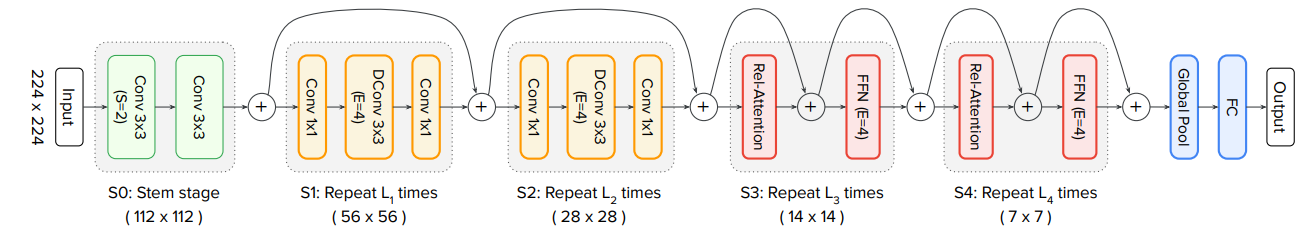
\includegraphics[width=\columnwidth]{figures/VisionTransformer/verticalDesign.png}
\end{figure}
\begin{itemize}
    \item Applying the relative-attention at pixel level is Computationally not possible
    \item A down-sampling of the image is needed
    \item Mimics CNNs architecture
\end{itemize}
\subsection{Relative self-Attention}
\begin{itemize}
    \item Combines Convolution and Attention
    \item Considers realitve position of tokens by introducing a global kernel value \(w_{i-j}\)
    \item  \textbf{Formula!}
\end{itemize}
	\section{Kolmogorov-Arnold Networks (KAN)}
The idea is to better approximate smooth functions with B-splines.

\subsection{B-Splines}
B-Splines are recursivly defined over a local area of knots(x coordinates)
Defined as \(B_{x-position,order}\).
\begin{figure}
    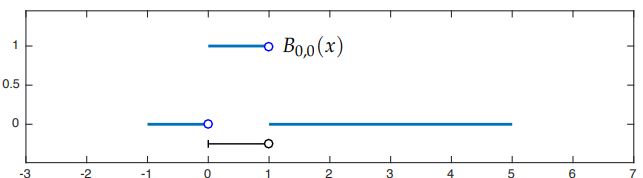
\includegraphics[width=0.5\columnwidth]{figures/KAN/BSplines1.png}
    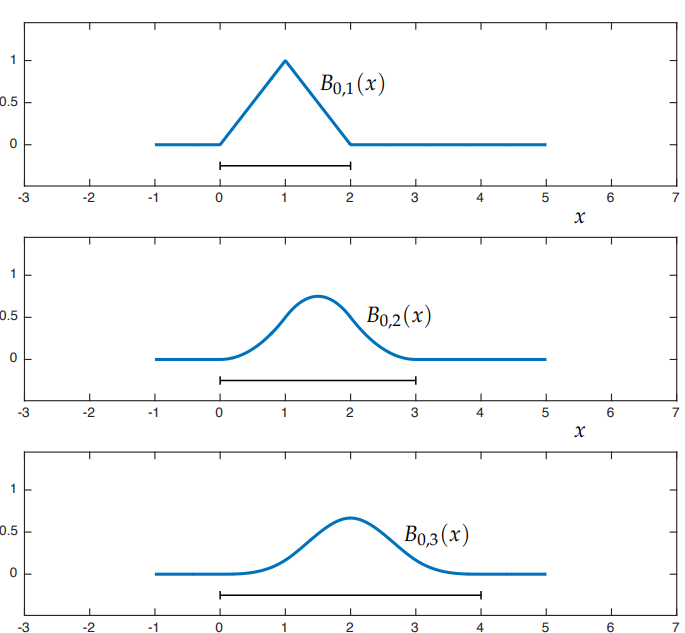
\includegraphics[width=0.5\columnwidth]{figures/KAN/BSplines2.png}
\end{figure}

\begin{figure}
    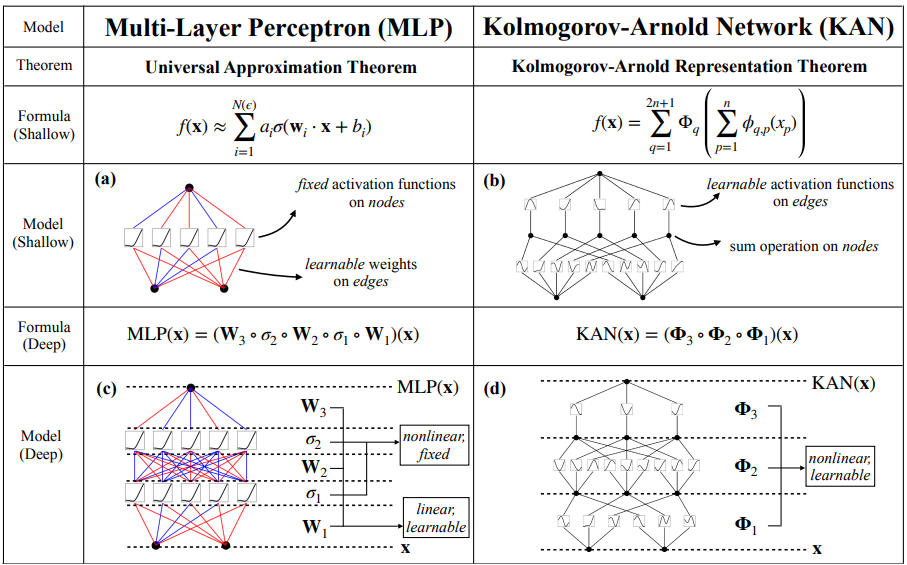
\includegraphics[width=\columnwidth]{figures/KAN/OverviewKANMLP.png}
\end{figure}
\begin{itemize}
    \item One main idea with the KANs is that they have better interpretability
    \item Aimed at math and physics applications
\end{itemize}
\subsection{Architecture}
\begin{itemize}
    \item Activation are on edges, not nodes, the nodes only do summation (no parameters)
    \item Non-linearity is applied on the edges before summing
\end{itemize}
	\section{Deep Reinforcement Learning 1 (Tabular Methods)}
\begin{figure}[!h]
    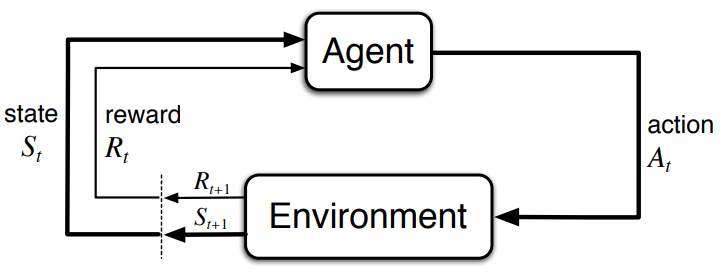
\includegraphics[width = 0.8\columnwidth]{figures/DeepReinforcementLearning1/EnvironmentAgent.png}
\end{figure}

Reinforcement Learning involves an agent interacting with an environment to learn decision-making. The agent:
\begin{itemize}
    \item Takes actions $A_t$ based on states $S_t$.
    \item Receives feedback in the form of rewards $R_t$.
    \item Learns to maximize cumulative rewards (return) $G_t$
\end{itemize}
cumulative reward or return (G):
\[
G_t = R_{t+1} + R_{t+2} + R_{t+3} + \dots + R_T
\]
Discounted return:
\[
G_t = R_{t+1} + \gamma R_{t+2} +\gamma^2 R_{t+3} + \dots = \sum_{k=0}^{\infty}\gamma^k R_{t+k+1}
\]
\begin{figure}[!h]
    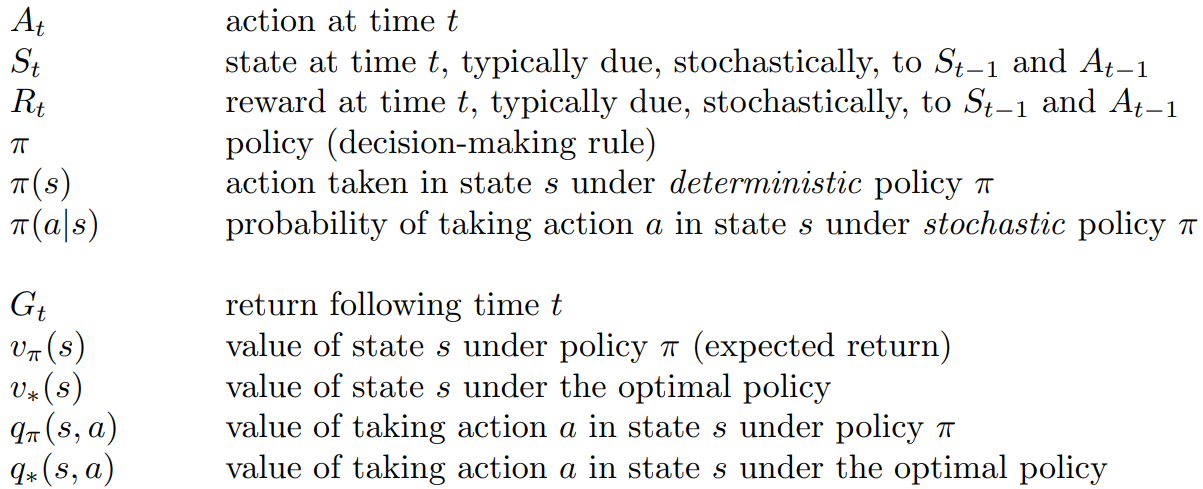
\includegraphics[width = \columnwidth]{figures/DeepReinforcementLearning1/OverviewNotation.png}
\end{figure}
\subsection{Formualtion of the Problem}
\begin{itemize}
    \item The actual value of an action \(a\) is the expected reward (which is not known)
    \[
    q_*(a) = \mathop{\mathbb{E}}[R_t|A_t = a]
    \]
    \item The estimated value of an action is called the (action-) value function \(Q_t(a)\) which we would like to be close to the true value
\end{itemize}
\subsubsection{Action-Value Mehtods}
\begin{itemize}
    \item Simple method(need to keep all rewards):
    \[
    Q_n = \frac{R_1 + R_2 +\dots + R_{n-1}}{n-1}
    \]
    \item Iterativ method:
    \[
    Q_{n+1} = Q_n + \frac{1}{n}(R_n - Q_n)
    \]
    \(R_n - Q_n\)(\(\left[Target- OldEstimation\right]\)) is like a Error.

\end{itemize}
This form
 \[\left[NewEstimation\leftarrow OldEstimation+StepSize\left[Error\right]
\right]\]
with different values for step and Error is used by many RL algorithm.
\subsection{Exploration vs Exploitation}
Exploitation:
\begin{itemize}
    \item Exploit current knowledge by taking  the action with the maximal estimated value
    \item Greedy action
\end{itemize}

Exploration:
\begin{itemize}
    \item Explore the value of other actions to get better estimates
    \item Non greedy actions
\end{itemize}
To balance Exploration and Exploitation:
\begin{itemize}
    \item \textbf{Exploitation:} With probability 1 - \(\epsilon\). Take greedy action with maximal \(Q_t(a)\)(greedy action)
    \item \textbf{Exploration:} With probability \(\epsilon\). Take any valid action with equal probability.
\end{itemize}
To use draw random variable in [0 .. 1].
Compare threshold with \(\epsilon\).
\begin{figure}[]
    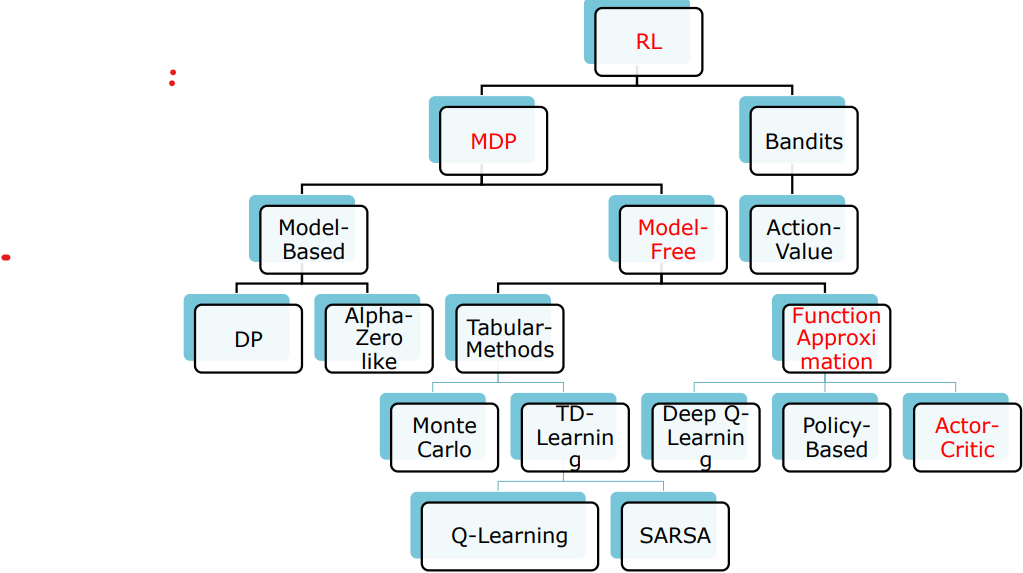
\includegraphics[width = \columnwidth]{figures/DeepReinforcementLearning1/RLOverview.png}
\end{figure}


\subsection{Mehtods Overview}

\subsection{Markov Decision Process (MDP)}
An MDP is defined by:
\begin{itemize}
    \item States $S$, actions $A$, and rewards $R$.
    \item Transition probabilities:
    \[
    p(s', r | s, a) = \Pr\{S_{t+1}=s', R_{t+1}=r | S_t=s, A_t=a\}
    \]
    \item Goal: Maximize the expected cumulative reward.
\end{itemize}

\subsection{Value Functions}
\subsubsection{State and Action-Value Functions}
\begin{itemize}
    \item State-value function under policy $\pi$:
    \[
    v_\pi(s) = \mathbb{E}_\pi[G_t | S_t = s]
    \]
    \item Action-value function under policy $\pi$:
    \[
    q_\pi(s, a) = \mathbb{E}_\pi[G_t | S_t = s, A_t = a]
    \]
\end{itemize}
\subsection{Policies}
A policy is a mapping from states to probabilities of selecting each possible action:
\[
\pi(a|s) = Pr\{A_t = a|S_t = s\}
\]
\subsubsection{Stochastic/Deterministic policies}
\begin{itemize}
    \item \textbf{Stochastic:} Different possible actions with different probabilities for each action. Example: rock, paper, scissor (1/3, 1/3, 1/3)
    \item \textbf{Deterministic:} Single action \(a\) is taken in a state \(s\).
\end{itemize}
\subsubsection{Bellman Equation}
For state-value function:
\[
v_\pi(s) = \sum_a \pi(a|s) \sum_{s', r} p(s', r | s, a) [r + \gamma v_\pi(s')]
\]
\subsection{Calculating the value function}
\begin{itemize}
    \item A solution to the value function for a policy can be found by solving the system of equations given by the Bellman equation for each state.
    \item If there are many states this system becomes large and computationally ineffective to calculate.
    \item We can solve it incrementally using Iterativ Mehtods (Dynammic Programming)
    \item However: Most often we do not have the Markov Decision Process given and have to explore the environment
\end{itemize}

\subsection{RL Algorithms: Value based methods}
\subsubsection{Monte-Carlo methods}
\begin{itemize}
    \item Monte-Carlo (MC) methods look at whole episodes and the average the complete results
    \item The task must be episodic
    \item Value estimations and policies are only changed \textbf{on the completion of an episode}
\end{itemize}

\subsubsection*{Monte Carlo Prediction}
\begin{itemize}
    \item We want to estimate \(v_\pi(s)\), the value of a state \(s\) under the policy \(\pi\).
    \item Given is a set of episodes.
    \item An episode might pass multiple times through\(s\), we will only consider it once, this is known as \textit{first-visit MC}.
    \item We average the retunrs of all episodes
\end{itemize}
\begin{figure}[!h]
    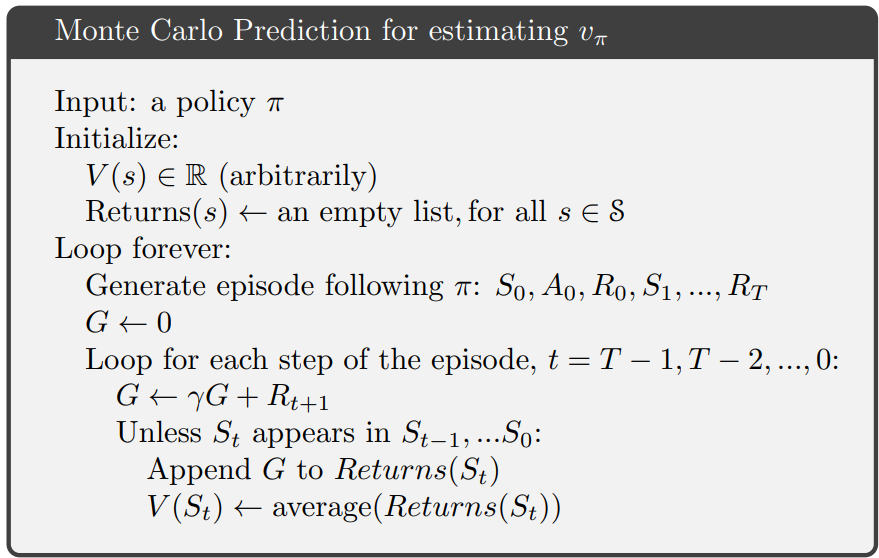
\includegraphics[width = \columnwidth]{figures/DeepReinforcementLearning1/MonteCarlo.png}
    \caption{Monte Carlo Prediction of the State-Value Function (first visit)}
\end{figure}

Intstead of averaging results, we would like an incremental calculation:
\[
    V(S_t) \leftarrow V(S_t) + \alpha[G_t - V(S_t)]
\]
If step size \(\alpha\) is \({1}/{n}\) its the same as averaging.

\subsubsection*{Policy Iteration:}
\begin{itemize}
    \item Knowing the state-value function will not help us to find a better policy, as we do not know which action will generate better returns
    \item Instead, we would like to predict the action-value function Q
    \item Given Q,we can find an improved policy by using greedy actions from Q 
    \item Using the new policy, we can predict its action-value function and repeat
    \item This is known as (generalized) policy-Iteration
\end{itemize}
\begin{figure}[!h]
    \centering
    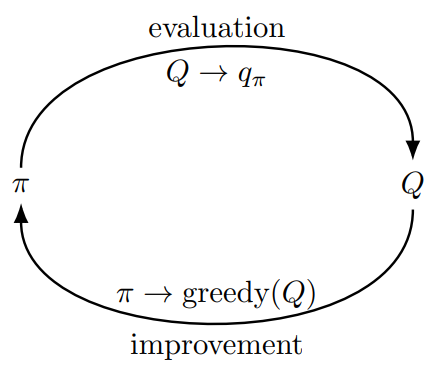
\includegraphics[width = 0.5\columnwidth]{figures/DeepReinforcementLearning1/PolicyIterationMonteCarlo.png}
\end{figure}

\subsubsection*{Exploration in MC}
\begin{itemize}
    \item We must maintain exploration to ensure that all state/action values are visited
    \item Out policy must be epsilon-soft:
    \item Each action in state must occur with a probability grater than zero
    \item 
\end{itemize}
\subsubsection{Temporal Difference (TD) Learning}
\begin{itemize}
    \item MC prediction with constant step size
    \[
    V(S_t) \leftarrow V(S_t) + \alpha[G_t - V(S_t)]
    \]

    \item TD methods make the update immediatly based on the estimates for the next state, which is just the application of the Bellman equation
    \[
    V(S_t) \leftarrow V(S_t) + \alpha[R_{t+1} + \gamma V(S_{t+1}) - V(S_t)]
    \]
\end{itemize}

\subsubsection*{SARSA (On-Policy TD Control)}
\begin{itemize}
    \item We use generalized policy iteration (GPI) for the control problem
    \item As in MC methods, we must balance exploration and exploitation 
    \item TD control methods generally learn an action-value function instead of a state-value function
    \item We look at the transition from (\textbf{S},\textbf{A}) with reward (\textbf{R}) to the next (\textbf{S},\textbf{A})(SARSA)
\end{itemize}
\[
Q(S_t, A_t) \leftarrow Q(S_t, A_t) + \alpha[R_{t+1} + \gamma Q(S_{t+1}, A_{t+1}) - Q(S_t, A_t)]
\]

\subsubsection*{Q-Learning (Off-Policy Control)}
\begin{itemize}
    \item SARSA uses teh Q-Values from the actual Action taken in the next step
    \item This action might not be the one, that maximizes the return
    \item While we cannot change the action taken, we can update the Action-Value using the best (or greedy) action from the next state, this is Q-Learning
\end{itemize}
\[
Q(S_t, A_t) \leftarrow Q(S_t, A_t) + \alpha[R_{t+1} + \gamma \max_a Q(S_{t+1}, a) - Q(S_t, A_t)]
\]
\begin{itemize}
    \item Q-Learning directly tries to approximate the optimal action-value function
    \item It uses a \textbf{soft policy} to determine which actions to take during the episode and the \textbf{greedy policy} to update the action-value estimates
    \item It is called a \textbf{off-policy} algorithm
\end{itemize}
\subsubsection*{Adaptaion}
\begin{itemize}
    \item \textbf{n-Step TD Prediction:} Instead of taking one step and then update the Q-Values we could take 2 or more Steps
    \item \textbf{Lamda-Returns:} Lamda-returns use a weighted sum of all the returns for the estimation
    \[
    G_t^\lambda = (1-\lambda)\sum_{n=1}^{\infty}\lambda^{n-1}G_{t:t+n}
    \]
\end{itemize}
\subsubsection{Summary value based methods}
\textbf{Monte Carlo Estimate:}
\begin{itemize}
    \item Calulate from one episode, estimate is sum of reward
    \item Multiple episode might go through the same state, the MC estimate is the average of those
    \item Estimate have \textbf{high variance}, as the estimates involve many (random) processes and decision along the entire episode
    \item They are \textbf{unbiased}
\end{itemize}
\subsubsection*{TD Estimate:}
\begin{itemize}
    \item A single reward is used and the estimate of the expected return from the next state (the estimate is using another estimate)
    \item Estimates of the next state will not be accurate early in the training
    \item Low variance, as you only depend on the next Steps
    \item Biased, because the estimate depends on the estimate of the next step, which might be inaccurate
\end{itemize}





	\section{Deep Reinforcement Learning 2 (Function Approximation)}
\begin{itemize}
    \item We want to approximate a state-values or the state-action-values by function that is parametrized by some paramer \textbf{w}.
    \[
    \hat{v}(s,\boldsymbol{w}) \approx v_\pi(s)
    \]
    \[
    \hat{q}(s,a,\boldsymbol{w}) \approx q_\pi(s,a)
    \]
    \item The dimensionality \(d\) of \textbf{w} will generally be much lower than the dimensionality of the state space
    \[
    d \ll |S|
    \]
    \item While there are many possibilities for function approximation, we will concentrate on \textbf{neural networks}
\end{itemize}
\subsubsection*{Prediction Objectiv}
As an objectiv, we would like to learn to approximate the value function at each state, so that the following error function is minimized:
\[
\left[v_\pi(s)-\hat{v}(s,\boldsymbol{w})\right]^2
\]
However, an update to one state, will affect the other state.
We want to introduce a function \(\mu(s)\) that measures how important each error is and then minimize the mean weighted error between the value function and its approximation.
\[
\overline{VE}(\boldsymbol{w}) = \sum_{s\in S}^{}\mu(s)\left[v_\pi(s)-\hat{v}(s,\boldsymbol{w})\right]^2
\]
(In practice,this just means that our samples are not distributed equally over all states.)
\subsection{Stochastic gradient descent}
\begin{itemize}
    \item Let us assume that in each step we observe a state \(s\) and its (true) value under the policy.
    \item We can use stochastic gradient-descent (SGD) to minimize the error in the observed examples
\end{itemize}
\begin{align*}
    \boldsymbol{w}_{t+1} &= \boldsymbol{w}_t - \frac{1}{2}\alpha\nabla\left[v_\pi(s)-\hat{v}(s,\boldsymbol{w})\right]^2\\
    &= \boldsymbol{w}_t + \alpha\left[v_\pi(s)-\hat{v}(s,\boldsymbol{w})\right]\nabla\hat{v}(S_t,\boldsymbol{w}_t)
\end{align*}
\begin{figure}[h]
    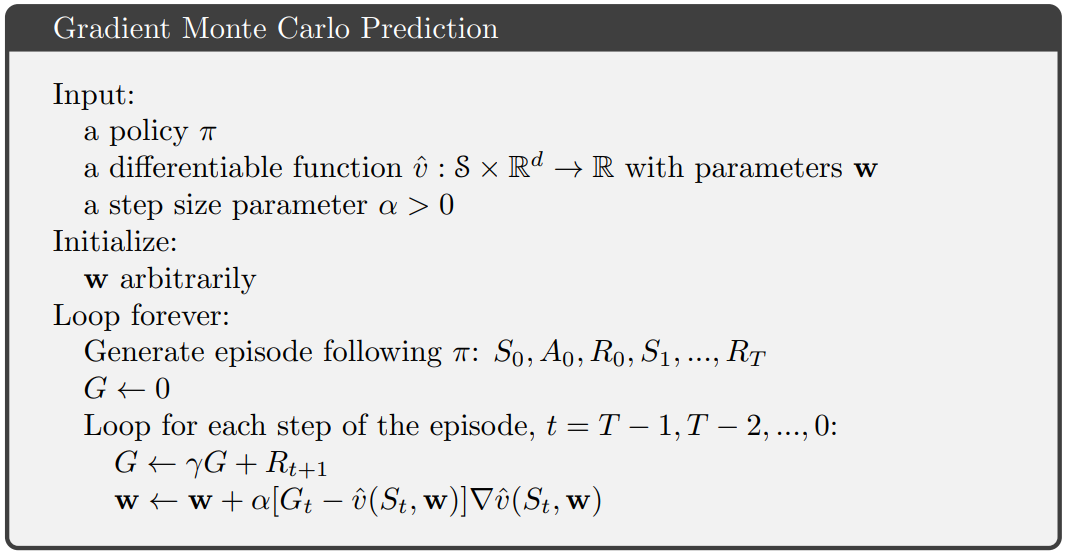
\includegraphics[width = \columnwidth]{figures/DeepReinforcementLearning2/GDMonteCarlo.png}
\end{figure}

\subsection{Deep Q-Learning}
\begin{figure}[!h]
    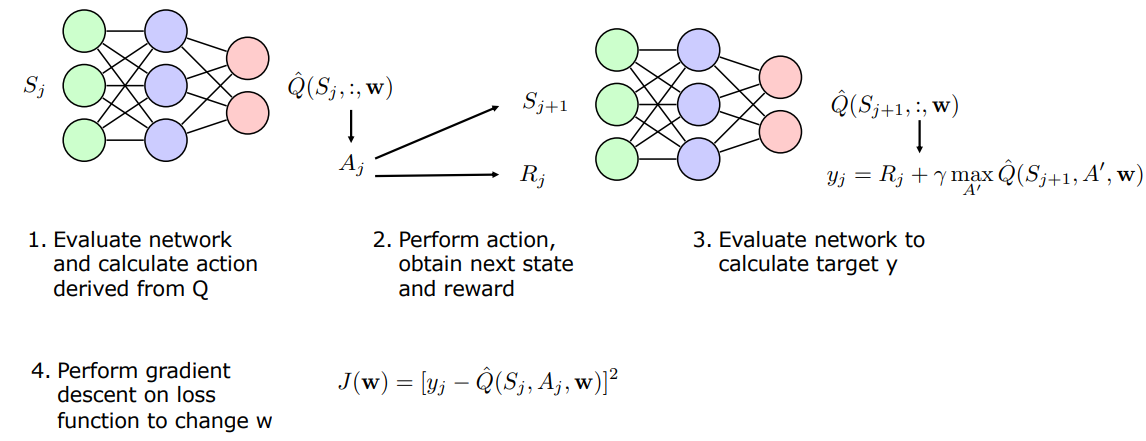
\includegraphics[width = \columnwidth]{figures/DeepReinforcementLearning2/BasicDeepQLearning.png}
\end{figure}
Use a neural network to approximate the Q-Function.
As multiple actions are needed to evaluate, multiple passes through the network are required.

A better approach is to use a neural network with inputs \(s\) to calculate the action-value function for all the actions simultaneously.
The output is a vector with a different q values for a given state.


\subsubsection{Problem: Moving Target}
\begin{itemize}
    \item As the calculation of the target function also depends on \textbf{w}, it will also be changed after a gradient step
    \item The target moves with every update to \textbf{w} while we are trying to approximate it.
    \item It is better to let the target remain stable, for this, another set of weights \(\boldsymbol{w}^-\) can be used that are updated after a few step.
\end{itemize}

\subsection{Experience Replay}
\begin{itemize}
    \item It is not efficient to update the network after one step
    \item Futhermore, a sample should be used more than once, similar to supervised learning, where we go over the data set multiple times
\end{itemize}
The \textbf{experience} at each time step is stored into a data set
\begin{align*}
    e_t &= (s_t, a_t, r_t, s_{t+1})\\
    D &= e_1, \dots, e_N
\end{align*}
\begin{itemize}
    \item A fixed size buffer is used that overwrites the oldest experience
    \item Training data then \textbf{sampled} from the data set
\end{itemize}
\begin{figure}[!h]
    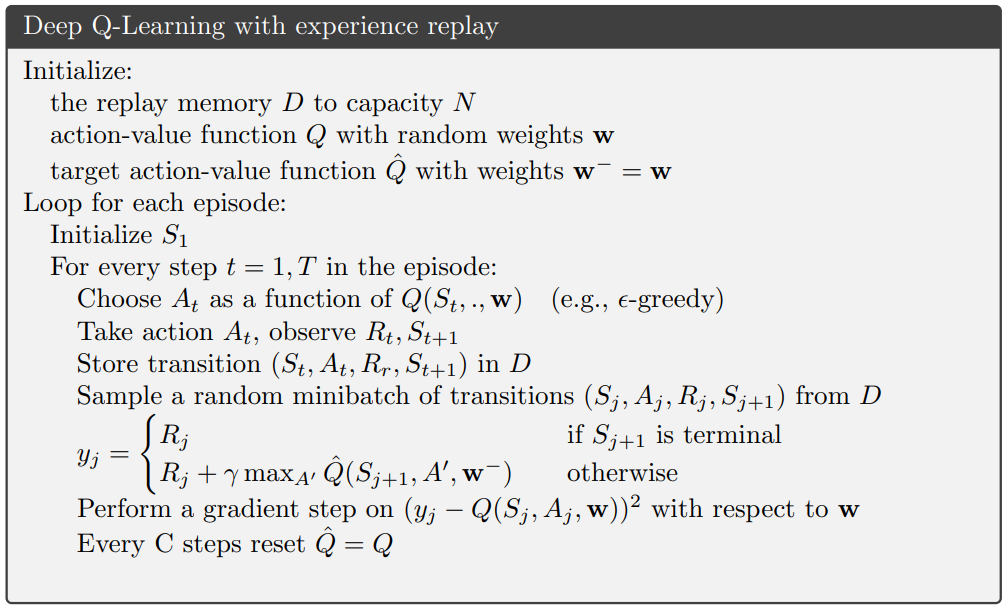
\includegraphics[width = \columnwidth]{figures/DeepReinforcementLearning2/DeepQLearningExperienceReplay.png}
\end{figure}

\subsection{Optimizing Deep Q-Learning}
Training for Deep Q-Learning is often difficult; several further concepts have been developed to make training easier:
\begin{itemize}
    \item Prioritized Experience Replay
    \item Double Q-Learning
    \item Dueling Networks
    \item Multi-step bootstrap targets
    \item Distributional DQN
    \item Noisy DQN
    \item Options of target weights update
\end{itemize}

\subsection{Policy Based Methods}
\begin{itemize}
    \item So far, all methods have been \textit{action-value methods}
    \item Policies were only calculated from those action-value estimates (using GPI)
    \item We now turn to methods that directly learn a parmetrized policy
    \[
    \pi(a|s,\boldsymbol{\theta}) = Pr\left\{A_t = a|S_t = s,\boldsymbol{\theta}_t = \boldsymbol{\theta}\right\}
    \]
    where \(\boldsymbol{\theta}\) are the parameters (weights) of the function that approximates the policy
\end{itemize}
\subsubsection*{Goal: Maximize Performance}
We want to change the weights, so that the return is maximized.
There are different algorithms to do that:
\begin{itemize}
    \item "Hill Climbing"
    \item Gradient Ascent
\end{itemize}

\subsubsection*{Policy Optimization with Hill Climbing}
Idea:
\begin{enumerate}
    \item Initialize weights for the function approximation arbitrarily
    \item Calculate the return \(G\) of an episode using the weights
    \item Change the weights slightly (add random noise)
    \item Calculate the return \(G\) using the new weights
    \item If return is larger: keep the new weights, decrease noise
    \item Otherwise: restore old weights, increase noise
    \item Continue with step 3
\end{enumerate}

\subsubsection{Why Policy-Based Methods}
\begin{itemize}
    \item While the goal of RL has been defiend is to maximize return \dots
    \item \dots we are not intrested in the actual value function, but
    \item \dots the \textbf{goal is to find the policy}
    \item Policy-based methods can learn true \textbf{stochastic policies}, this is different from epsilon greedy methods which add randomness just exploration
    \item Aliased states: States that look similar (same observation) but are actually different are difficult to handle with deterministic policies
    \item Finding the optimal action in values-based methods is difficult for continuous action spaces
\end{itemize}

\subsection{Policy Gradient Methods}
\begin{itemize}
    \item \textbf{Policy-based methods:} Search for optimal policy
    \item \textbf{Policy gradient methods:} Use \textbf{gradient ascent} to find the best parameters (Requires the approximation function to be differentiable)
    \[
    \boldsymbol{\theta}_{t+1} = \boldsymbol{\theta} + \alpha \widehat{\nabla J(\boldsymbol{\theta})}
    \]
    where
    \[
    \widehat{\nabla J(\boldsymbol{\theta})}
    \]
    is a stochastic estimate of the gradient of the performance measure.
\end{itemize}

\subsubsection*{Constrains for the policy}
The policy should be a probability function over the different actions and must use exploration, therefor:
\begin{itemize}
    \item The probability of any action should be greater than 0:
    \[
    \pi(a|s,\boldsymbol{\theta}) > 0, \text{for all } a \in A,s \in S
    \]
    \item The sum of all probabilities must be 1:
    \[
    \sum_{a}^{}\pi(a|s,\boldsymbol{\theta}) = 1, \text{for all } s \in S
    \]
    \item Use action-preferences and softmax:
    \[
    h(s,a,\mathbf{\theta})\in\mathbb{R} \qquad \pi(a|s,\boldsymbol{\theta}) = \frac{e^{h(s,a,\boldsymbol{\theta})}}{\sum_{b}^{e^{h(s,b,\boldsymbol{\theta})}}}
    \]
\end{itemize}

\subsubsection*{Episodic case}
\begin{itemize}
    \item Goal: optimize the total return from a (particular) state
    \[
    J(\boldsymbol{\theta}) = v_{\pi\boldsymbol{\theta}}(s_0)
    \]
    \item Problem: v depends on action selection and state distribution
    \item Policy gradient theorem:
    \[
    \nabla J({\boldsymbol{\theta}})\propto \sum_{s}^{}\mu(s)\sum_{a}^{}q_\pi(s,a)\nabla\pi(a|s,\boldsymbol{\theta})
    \]
\end{itemize}

\subsubsection*{REINFORCE: Monte Carlo Policy Gradient}
\begin{itemize}
    \item Update the weights according to:
    \begin{align*}
        \boldsymbol{\theta}_{t+1} &= \boldsymbol{\theta} + \alpha G_t\frac{\nabla\pi(A_t|S_t,\boldsymbol{\theta})}{\pi(A_t|S_t,\boldsymbol{\theta})}\\
        &= \boldsymbol{\theta} + \alpha G_t\nabla ln\pi(A_t|S_t, \boldsymbol{\theta})
    \end{align*}
    \item The second line can be derived from
    \[
    \nabla ln(f(x)) = \frac{\nabla f(x)}{f(x)}
    \]
    \item This is gradient \textbf{ascent}, as we want to maximize the return
\end{itemize}
\subsubsection*{How policy gradient works}
\begin{itemize}
    \item After the episode is complete, the policy gradient algorithm will look at each state and consider the selected action.
    \item If the return G was to high, it will make the action more likely
    \item If the return was low, it will reduce the probability
\end{itemize}

\subsubsection*{Problems with REINFORCE}
Policy Gradient is Noisy!
\begin{itemize}
    \item Gradient should be over millions episodes or trajectories (truncated episodes)
    \item But we typically only use one trajectory
    \item We should generate a number of trajectories, and calculate the trajectory from them 
    \item We can then also reduce noise by calculating the mean and standard deviation of the samples by reward normalization, this is called batch normalization
\end{itemize}

\subsubsection*{Baseline}
A "trick" for faster convergence and less variance is to subtract a baseline from the q values, where the baseline can be any function that does not depend on the action
\[
\nabla J({\boldsymbol{\theta}})\propto \sum_{s}^{}\mu(s)\sum_{a}^{}(q_\pi(s,a)-b(s))\nabla\pi(a|s,\boldsymbol{\theta})
\]
\[
    \boldsymbol{\theta}_{t+1} = \boldsymbol{\theta} + \alpha (G_t-b(S_t))\frac{\nabla\pi(A_t|S_t,\boldsymbol{\theta})}{\pi(A_t|S_t,\boldsymbol{\theta})}
\]
\begin{itemize}
    \item A natural choice for b, is to estimate a state value
    \[
    \hat{v}(S_t,\boldsymbol{w})
    \]
    \item where the weights would also be learned using the Monte-Carlo method
    \item The function is not dependent on the policy parametrization, so the gradient remains the same
    \item The difference between q and v is also called the \textit{advantage} function:
    \[
    q(s,a) - v(s)
    \]
\end{itemize}

\subsubsection*{Why does this baseline help?}
\begin{itemize}
    \item The current policy is used to sample actions, while the policy is also update from observations from the same actions.
    \item This creates an exploration-exploitation dilemma
    \item With a value baseline, the aggressiveness of the updates is reduced
\end{itemize}
\subsubsection{Summary Policy Gradient Methods}
Advantages:
\begin{itemize}
    \item Often better convergence properties
    \item Effective in high dimensional or continuous action spaces
    \item Can learn stochastic policies
\end{itemize}
Disadvantages:
\begin{itemize}
    \item Typically converge to local rather than global optimum
    \item Evaluating a policy can be inefficient and high variance
\end{itemize}
\subsubsection*{More on policy gradient Methods}
\begin{itemize}
    \item This was the \textit{vanilla} policy gradient method
    \item There are variations regarding the update and the sampling that make the methods more stable and faster to converge
    \item These are the Trust Region Policy Optimization (TRPO) and the Proximal Policy Gradient (PPO) methods
\end{itemize}

\subsection{Actor-Critic Methods}
1-step Policy Gradient Method with Critic
\begin{itemize}
    \item We would like to implement a 1-step (or n-step) method like TD(0) for the policy
    \item However, we then need a \textbf{value} function, so we can replace the full return in REINFORCE with the 1-step return:
    \begin{align*}
        \boldsymbol{\theta}_{t+1} &= \boldsymbol{\theta}_t + \alpha(R_t + \gamma\hat{v}(S_{t+1},\boldsymbol{w})-\hat{v}(S_t,\boldsymbol{w}))\nabla \text{ln}\pi(A_t|S_t,\boldsymbol{\theta}_t)\\
        &= \boldsymbol{\theta}_t + \alpha\delta_t\nabla \text{ln}\pi(A_t|S_t,\boldsymbol{\theta}_t)
    \end{align*}
    \item The policy is called the \textit{actor}, the value function the \textit{critic}
    \item The value function approximation can be calculated as in deep Q-Learning
\end{itemize}
\begin{figure}[!h]
    \centering
    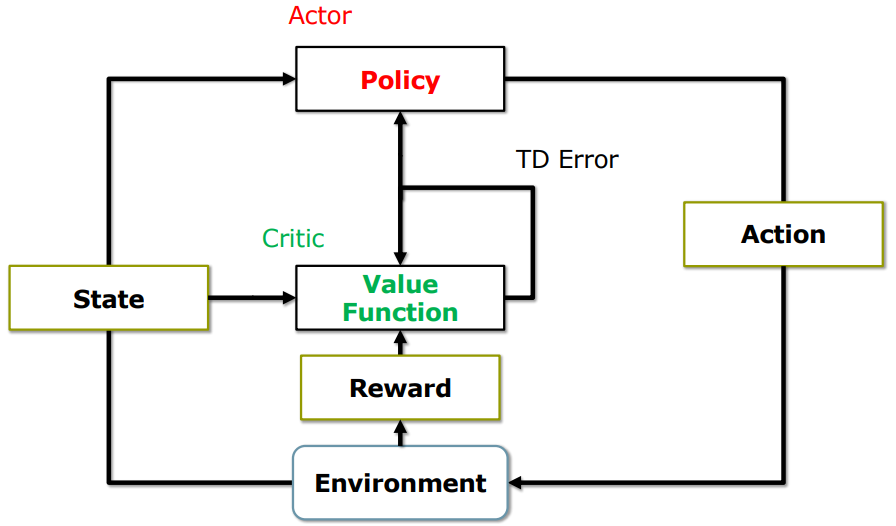
\includegraphics[width = \columnwidth]{figures/DeepReinforcementLearning2/ActorCritic.png}
\end{figure}

\subsection{Overview: Value and Policy based Methods}
Value Based:
\begin{itemize}
    \item Learnt Value Function
    \item Implicit Policy (e.g. epsilon greedy)
\end{itemize}
Policy Based:
\begin{itemize}
    \item No Value Function
    \item Learnt Policy
\end{itemize}
Actor-Critic
\begin{itemize}
    \item Learnt Value Function
    \item Learnt Policy
\end{itemize}

\subsubsection*{Example: How to play tennis?}
Policy based(REINFORCE):
\begin{itemize}
    \item Play matches
    \item Think about the matches that you won and lost, and do more of the actions you did in the won matches and less of those in the lost matches
\end{itemize}
Value based
\begin{itemize}
    \item You guess what the score will be like (during the match) and select actions that maximize the score
    \item Guesses get better, resulting in better performance
    \item but guesses can be wrong(biased, prone to over or underestimate)
\end{itemize}
Actor-Critic based:
\begin{itemize}
    \item Combine both approaches
    \item Actor Critic methods are more stable than value-based agents and need fewer samples than policy-based approaches
\end{itemize}
\subsubsection*{Different Actor-Critic/Policy Gradient Methods}
There are different choices for the value of \(\psi\) in the expression for the gradient:
\[
\psi \nabla_{\boldsymbol{\theta}} \text{ln}\pi(A_t|S_t,\boldsymbol{\theta})
\]
\begin{table}[!h]
    \begin{tabular}{lr}
    \(\psi = G\)    &  Return from episode\\
    \(\psi = Q(A_t,S_t)\)     &  Action-value function\\
    \(\psi = A(A_t,S_t)\)     &  Advantage function\\
    \(\psi = r_t + V(S')-V(S)\)     & TD(0) residual
    \end{tabular}
\end{table}
	\section{Deep Reinforcement Learning 1 (Use Deep RL)}
\subsubsection*{Goal}
\begin{itemize}
    \item Which algorithm to take
    \item Which framework do exist
    \item Which hyperparameter are most important to get right first
    \item How to design environment and rewards
\end{itemize}
\subsection{Frameworks}
\subsubsection*{OpenAI gym / gymnasium}
\begin{itemize}
    \item Not really a framework for RL Algorithms, but for the \textbf{environment}
    \item Many other frameworks use the gym environment model or build upon the same interface
    \item Contains useful utilities and wrappers
    \item Contains many standard benchmark environments
\end{itemize}
\subsubsection*{Stable Baseline 3}
\begin{itemize}
    \item Contains reliable implementation of basic RL algorithms
    \item Relative beginner friendly
    \item Less efficient and parametrized than other frameworks
\end{itemize}
\subsubsection*{RLLIB on Ray}
\begin{itemize}
    \item Large collection of algorithms
    \item Able to provide own implementation of models and algorithms
    \item Builds upon ray and ray.tune for distributed workflows
    \item More advanced and difficult to use (or debug)
    \item Our framework of choice for research problems that require complex algorithms and days of training
\end{itemize}
\subsubsection*{Spinning up}
Educational resource to make it easier to learn RL.

\subsection{Optimizing Deep Q-Learning}
Training for Deep Q-Learning is often difficult; several further concepts have been developed to make training easier:
\begin{itemize}
    \item \textbf{Prioritized Experiance Replay}
    \item \textbf{Double Q-Learning}
    \item \textbf{Dueling Networks}
    \item Multi-step boostrap target
    \item Distributional DQN
    \item Noisy DQN
    \item \textbf{Target weights updates}
\end{itemize}

\subsubsection{Prioritized Experiance Replay}
Idea:
\begin{itemize}
    \item An agent should be able to learn more efficiently from transitions than from others
    \item By what criterion can we measure the importance of each transition
\end{itemize}
\textbf{TD error} indicates how surprising or unexpected the transition is, so samples with a high TD error should be prioritizd.
However:
\begin{itemize}
    \item Only using the prioritized transition can lead to errors too 
    \item Use stochastic sampling and the priority as weights for the probability
\end{itemize}
\subsubsection*{Calculating Priorities}
Calculate Priorities from TD Errors:
\begin{itemize}
    \item Take the magnitude of the TD Error as Priority
    \item Store the priorities with each corresponding tuple in the replay buffer
    \item Compute sampling probabilities when creating the batches
\end{itemize}
TD Error is Zero:
\begin{itemize}
    \item If the TD Error is zero, the priority will also be zero
    \item To prevent tuples from starving, we can add a small constant
    \[
    p(i) = |\delta_i| + epsilon
    \]
\end{itemize}
\subsubsection*{Prioritized Experience Replay: Sampling}
The probability of sampling a transition \(i\) is
\[
P(i) = \frac{p_i^\alpha}{\sum_{k}^{}p_k^\alpha}
\]
the parameter \(\alpha\) is another hyperparameter that controls the influence of priority values:
\begin{itemize}
    \item if it is equal to 0, the priorities are ignored, and uniform sampling is used
    \item if it is 1, only the priorities are used
\end{itemize}

\subsubsection{Double Q-Learning}
\begin{itemize}
    \item Q-Learning is known to overestimate action-values under certain conditions
    \item The Q function is used in both to \textbf{select the best action} and to \textbf{evaluate} it:
    \[
    y_j^{DQN} = R_j + \gamma Q(S_{j+1},\text{arg}\max_a Q(S_{j+1},a,\boldsymbol{w}),\boldsymbol{w})
    \]
    \item In the early stages of learning, the Q function can be noisy, then a possible wrong Q value can be increased too much
    \item Overestimating can be diminished by using a second function approximation:
    \[
    y_j^{DoubleDQN} = R_j + \gamma Q(S_{j+1},\text{arg}\max_a Q(S_{j+1},a,\boldsymbol{w}),\boldsymbol{w}')
    \]
    \item now the value is only increased if the Q value is high in both approximations
    \item Where do we get another function approximation from?
    \item In DQN we already use two networks and \(w^-\) is significantly different enough from \(w\) to be used:
    \[
    y_j^{DoubleDQN} = R_j + \gamma Q(S_{j+1},\text{arg}\max_a Q(S_{j+1},a,\boldsymbol{w}),\boldsymbol{w}^-)
    \]
\end{itemize}
\subsubsection{Dueling Networks}
The idea behind dueling networks is to use a \textbf{two-headed} network that branches into head each for calculating:
\begin{itemize}
    \item The \textbf{value} function
    \item The \textbf{advantage} function
    \item The sum of the two function will give the action-value function, as
    \[
    Q(s,a) = V(s) + A(s,a)
    \]
\end{itemize}
\begin{figure}[!h]
    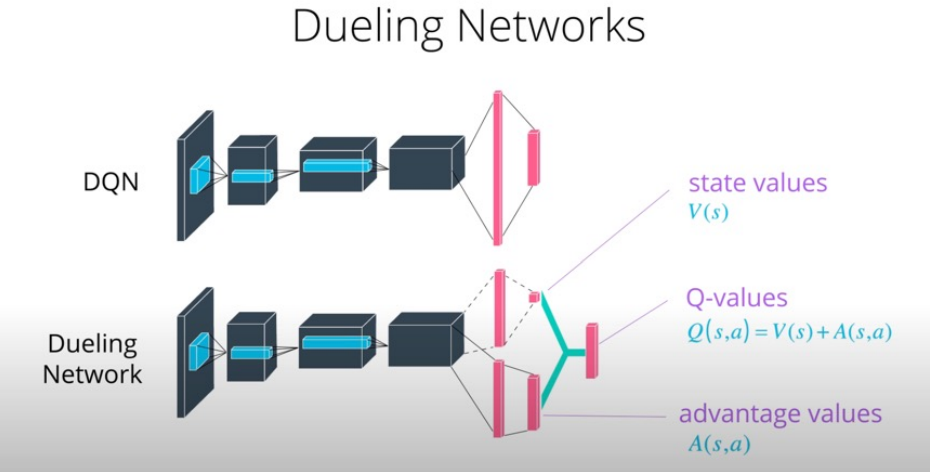
\includegraphics[width = \columnwidth]{figures/DeepReinforcementLearning3/DuelingNetworks.png}
\end{figure}
\subsubsection{Update of target weights}
A different set of weights are used for the target function on DQN, than the one that is trained.
This set must be updated with the trained version.

Update strategie:
\begin{itemize}
    \item Update after n training steps (original DQN)
    \item Update by linear interpolation between target and current weights (often works better)
    \[
    w^- = \tau w + (1-\tau)w^-
    \]
\end{itemize}
\subsubsection{Trust Region Policy Optimization (TRPO)}
In policy gradient methods, the update is calculated as
\[
\boldsymbol{\theta}_{t+1} = \boldsymbol{\theta}_t + \alpha\nabla J(\boldsymbol{\theta})|_{\boldsymbol{\theta} = \boldsymbol{\theta}_t}
\]
The new values for \(\theta\) should be near to the old values, as we use a small step size, however, the \textbf{policy} could still change significantly with a change of \(\boldsymbol{\theta}\).

We would like to make sure that the \textbf{new and old policies} are not too far apart (not that only the parameters are close)
\subsubsection*{Trust Region Policy Optimization}
\begin{itemize}
    \item We would like to compare the policies, but these are distributions (probabilities for each action)
    \item We can use the Kullback-Leiber divergence (KL-divergence), this is a common measure to compare distributions
    
    \[
    D_{KL}(P||Q) = \sum_{x}^{}P(x) \text{log}\frac{P(x)}{Q(X)}
    \]
\end{itemize}

We can write the cost function as a function of two policies and optimize that
\[
J(\boldsymbol{\theta},\boldsymbol{\theta}_t) = \mathbb{E}_{a~\pi}\left[\frac{\pi_{\boldsymbol{\theta}}(a|s)}{\pi_{\boldsymbol{\theta}_t}(a|s)}A(s,a)\right]
\]
i.e. this measures how the new policy performs relative to the old policy, then we find 
\[
    \boldsymbol{\theta}_{t+1} = \text{arg}\max_{\boldsymbol{\theta}} J(\boldsymbol{\theta},\boldsymbol{\theta}_t)
\]
under the constrained
\[
D_{KL}(\boldsymbol{\theta}_{t+1}||\boldsymbol{\theta}_t) \le \delta
\]
\begin{itemize}
    \item So we maximize the so-called surrogate performance function:
    \[
    J(\boldsymbol{\theta},\boldsymbol{\theta}_t)
    \]
    \item Actual implementation is mathematically a bit more complicated
    \item A Taylor approximation of the objectiv and the constraint is used
    \item As this approximation requires to inverse a matrix (which is very expensiv for the many parameters of a neural network), the constraint problem of optimization is solved by approximate solutions (conjugate gradient)
    \item The idea behind TRPO and using the surrogate performance functions are good, but tha algorithm is inefficient \(\rightarrow\) PPO
\end{itemize}
\subsubsection{Proximal Policy Gradient (PPO)}
\begin{itemize}
    \item PPO tries to solve the same problem but uses clipping instead of constraint on the KL-divergence
    \item Enforcing a constraint can also be viewed as imposing a penalty when the function gets near to it
    \item So there are two variants of PPO, with clippingor with a penalty
    \item We will show a deriviation of PPO from the additional viewpoint of trajectory sampling
\end{itemize}
\subsubsection*{Policy Update in REINFORCE}
\begin{figure}
    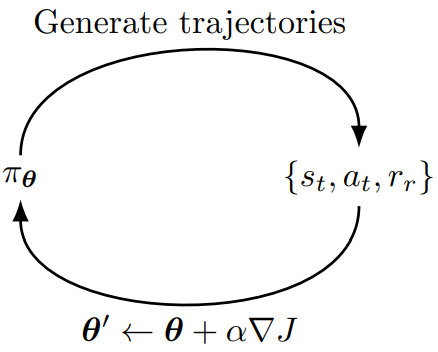
\includegraphics[width = 0.5\columnwidth]{figures/DeepReinforcementLearning3/PPOPolicyUpdate.png}
\end{figure}
\begin{itemize}
    \item The policy is used to generate a trajectory (episodes or part of one)
    \item The trajectory is then used to calculate the gradient and update the policy
    \item So, the just sampled trajectories do not correspond to actual policy
    \item Sampling trajectories is computing intensive: Could we recycle old trajectories?
\end{itemize}
\subsubsection*{Importance Sampling}
To calculate any experience values, we need to incorporate the probability of the trajectory:
\begin{equation*}
    \sum_{\tau}^{}P(\tau;\boldsymbol{\theta}')R(\tau)
\end{equation*}

\begin{equation*}
    \sum_{\tau}^{}P(\tau;\boldsymbol{\theta})\frac{P(\tau;\boldsymbol{\theta}')}{P(\tau;\boldsymbol{\theta}')}R(\tau)
\end{equation*}
\(P(\tau;\boldsymbol{\theta})\) is the old policy.
\(\frac{P(\tau;\boldsymbol{\theta}')}{P(\tau;\boldsymbol{\theta}')}R(\tau)\) is the Re-weight factor.
So we can use old trajectories if we weight the sample according to the re-weighting factor.
\subsubsection*{Re-weighting factor}
\[
\frac{P(\tau;\boldsymbol{\theta}')}{P(\tau;\boldsymbol{\theta})} = \frac{
    \pi_{\boldsymbol{\theta}'}(a_1|s_1) \pi_{\boldsymbol{\theta}'}(a_2|s_2) \pi_{\boldsymbol{\theta}'}(a_3|s_3) \dots
}{
    \pi_{\boldsymbol{\theta}}(a_1|s_1) \pi_{\boldsymbol{\theta}}(a_2|s_2) \pi_{\boldsymbol{\theta}}(a_3|s_3) \dots
}
\]
\begin{itemize}
    \item Can easily be close to zero or infinity if any of the policies become close to 0
    \item We would like to ensure that this factor remains close to 1
\end{itemize}
\subsubsection*{Re-weighting Policy Gradient}
\begin{equation*}
        g = \underbrace{\nabla_{\boldsymbol{\theta}'}\sum_{t}^{}\frac{
    \pi_{\boldsymbol{\theta}'}(a_t|s_t)
    }{
    \pi_{\boldsymbol{\theta}}(a_t|s_t)
    }R_t}_{L_{sur}}
\end{equation*}
\begin{equation*}
    g = \nabla_{\boldsymbol{\theta}'}L_{sur}(\boldsymbol{\theta}',\boldsymbol{\theta})
\end{equation*}
\begin{equation}
    L_{sur}(\boldsymbol{\theta}',\boldsymbol{\theta}) = \nabla_{\boldsymbol{\theta}'}\sum_{t}^{}\frac{
        \pi_{\boldsymbol{\theta}'}(a_t|s_t)
        }{
        \pi_{\boldsymbol{\theta}}(a_t|s_t)
        }R_t
\end{equation}
This is only valid, if the old and the new policy is similar.

\subsubsection{PPO: Clipped Objective}
CPI: Conservative Policy Iteration 
\begin{equation*}
    L^{CPI}(\boldsymbol{\theta}) = \mathbb{E}_t\left[\frac{
        \pi_{\boldsymbol{\theta}}(a_t,s_t)
        }{
            \pi_{\boldsymbol{\theta}(a_t|s_t)}
        }A_t\right] = \mathbb{E}_t\left[r_t(\boldsymbol{\theta})A_t\right]
\end{equation*}
\begin{equation*}
    L^{CLIP} = \mathbb{E}_t\left[
        \min(r_t(\boldsymbol{\theta})A_t,clip(r_t(\boldsymbol{\theta}),1-\epsilon,1+\epsilon))
    \right]
\end{equation*}
\begin{equation*}
    \boldsymbol{\theta}_{k+1} = \text{arg}\min_{\boldsymbol{\theta}}\mathbb{E}_t\left[
        \min(r_t(\boldsymbol{\theta})A_t,clip(r_t(\boldsymbol{\theta}),1-\epsilon,1+\epsilon))
    \right]
\end{equation*}
\begin{figure}[!h]
    \centering
    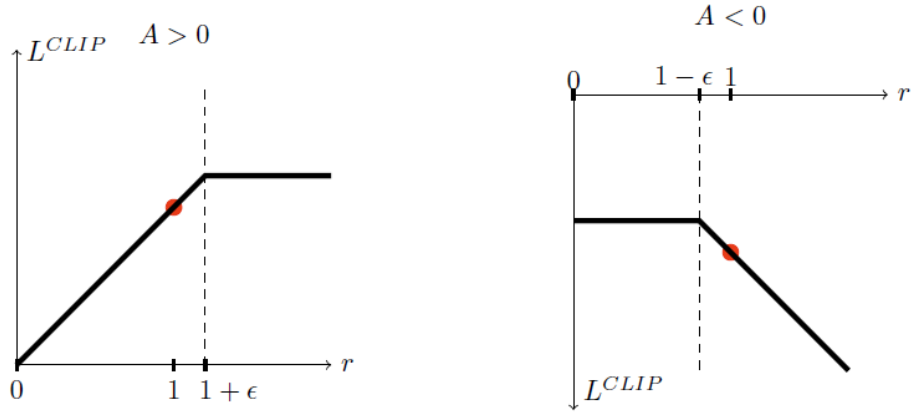
\includegraphics[width = 0.5\columnwidth]{figures/DeepReinforcementLearning3/PPOClip.png}
\end{figure}
\subsubsection*{PPO Summary}
\begin{itemize}
    \item By adjusting the step size in the update of the weights, we can ensure that the weights do not change too much
    \item However, even a small change in the weights could be a large change in the policy
    \item We would like to ensure, that the policy does not change too much
    \item In PPO, we enforce that the ratio of the new to old policy stays within 
    \[
    \left[1-\epsilon,1 + \epsilon\right]
    \]
\end{itemize}
\subsection{Asynchronous Advantage Actor-Critic (A3C)}
\begin{figure}[h!]
    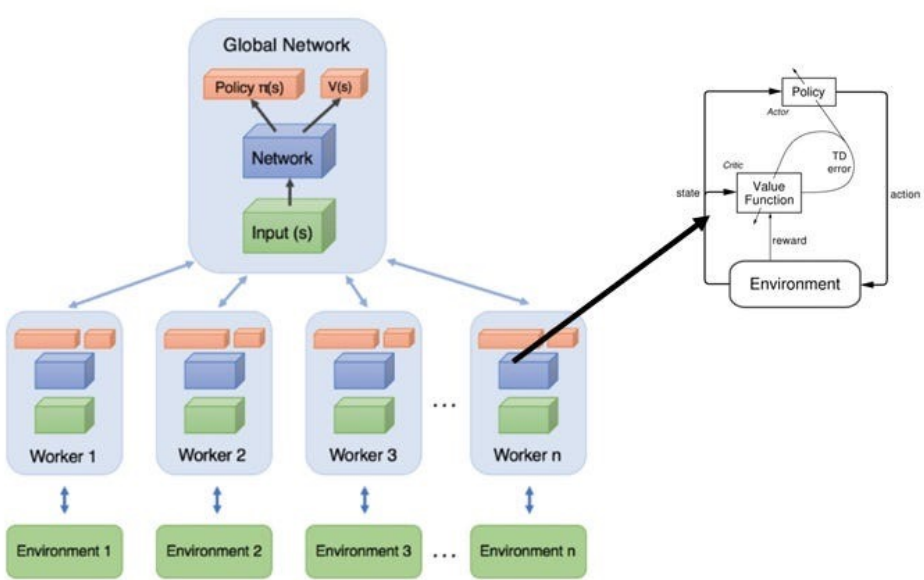
\includegraphics[width = \columnwidth]{
        figures/DeepReinforcementLearning3/A3C.png
    }
\end{figure}
Idea:
\begin{itemize}
    \item Use multiple workers
    \item Fixed length segments of experience to compute estimates of the return and advantage function
\end{itemize}
Asynchronous update:
\begin{itemize}
    \item Each agents updates the training network at its own time and independently
    \item Experience might come from older network copies of the other agents as well
    \item Data is uncorrelated, as the agents have different behaviors
    \item Allows on-policy training, which is more stable
\end{itemize}
\subsection{Advantage Actor-Critic (A2C)}
\begin{figure}[h!]
    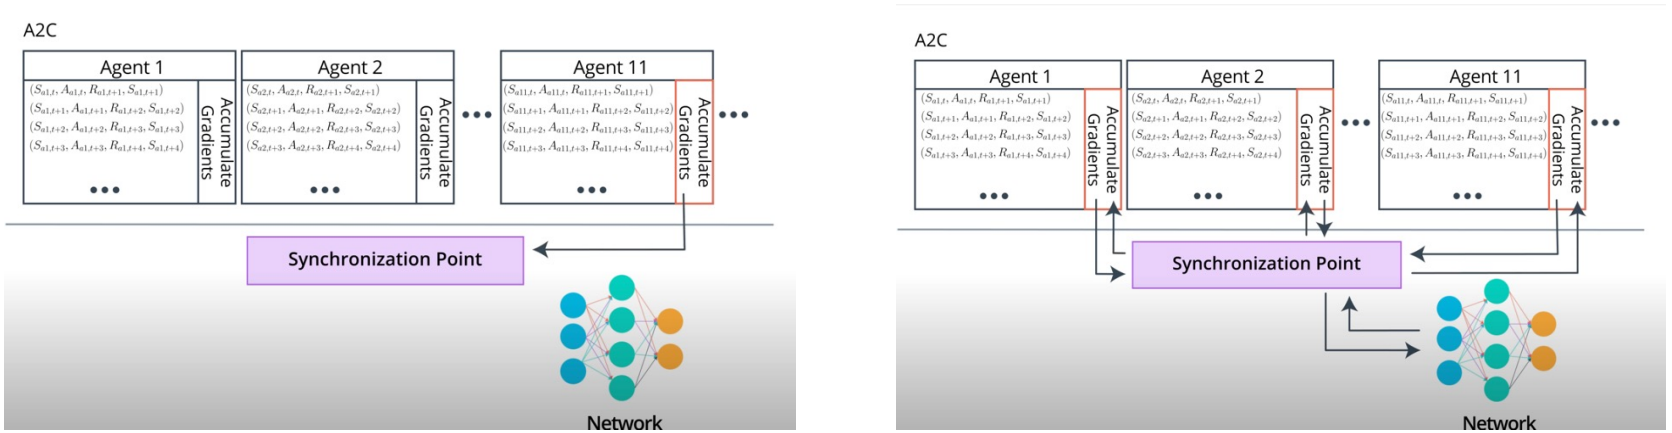
\includegraphics[width = \columnwidth]{
        figures/DeepReinforcementLearning3/A2C.png
    }
\end{figure}
Asynchronous doesnt improve performance.
It is also possible to use multiple workers, but wait until all workers have finished their episodes and then calculate an average gradient for the training step.
	\section{Graph Neural Networks 1}
Graphs and machine learning:
\begin{itemize}
    \item How to take advantage of the relational structure for better prediction?
    \item Many Deep Learning Approaches are designed for sequential data or grid data.
    \item Networks are more complex: Graph Deep Learning is harder
\end{itemize}
\subsection{Definition of a(heterogenous) Graph}
\(G = (V,E,R,T)\)
\begin{table}[!h]
    \begin{tabular}{lr}
    Nodes with node types    &  \(v_i \in V\)\\
    Edges with relation types     &  \((v_i,r,v_j) \in E\)\\
    Node type     &  \(T(v_i)\)\\
    Relation type     & \(r \in R\)
    \end{tabular}
\end{table}
Directed or undirected Edges
\subsection{Heterogenous Graphs}
\begin{figure}[!h]
    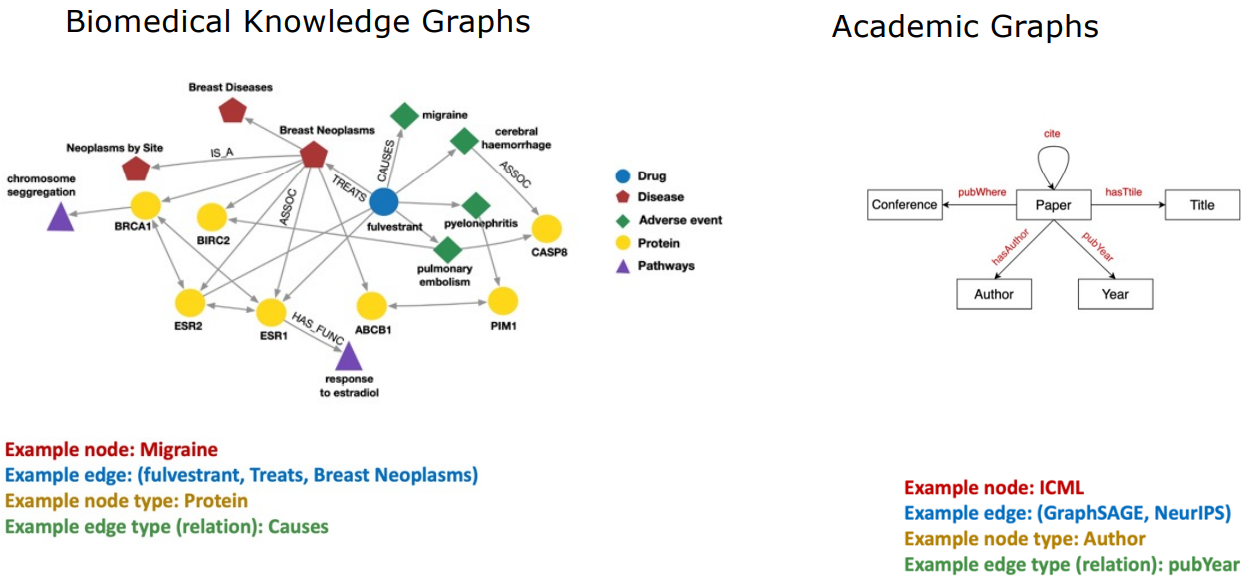
\includegraphics[width = \columnwidth]{figures/GraphNeuralNetworks1/HeterogenousGraphExample.png}
\end{figure}

\subsection{Tasks on Graphs}
Many of the problems that we would like to solve, can be described as one of several taks on graphs:
\begin{itemize}
    \item Node Level Tasks
    \item Edge Level Tasks
    \item Graph Level Tasks, Prediction / Generation
    \item Community (Subgraph) Level Taks
\end{itemize}

\subsubsection{Node Level Tasks}
Predict the identity of node in the graph.
Karate club: Predict if the student becomes loyal to Mr.Hi or Mr.John A.
\subsubsection*{Examples:}

Predict a proteins 3D structure based on its amino acid sequence:
For each node: Predict its 3D coordinates

AlphaFold:
\begin{itemize}
    \item Key idea: Spatial Graph 
    \item \textbf{Nodes:} Amino acids in a protein sequence 
    \item \textbf{Edges:} Proximity between amino acids (residues) 
\end{itemize}

\subsubsection{Edge Level Tasks}
Predict or label edges 
\subsubsection*{Examples}
Recommender System:
\begin{itemize}
    \item User interacts with items:
    \subitem Watch movies, buy merchandise, listen to music
    \item Nodes:
    \subitem Users and items
    \item Edges
    \subitem User-item interactions 
\end{itemize}
\begin{figure}[!h]
    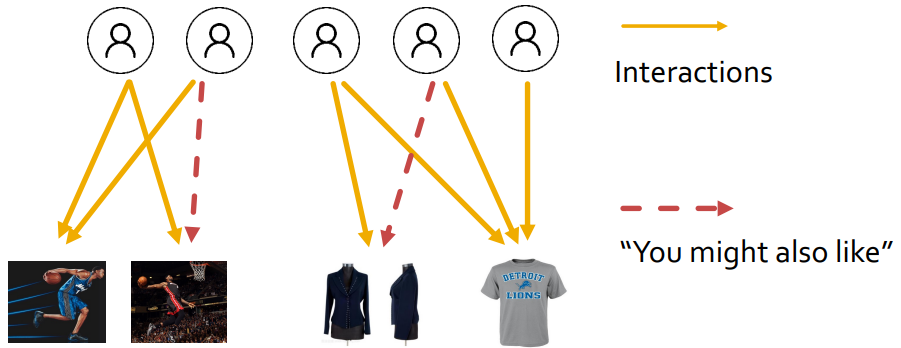
\includegraphics[width = \columnwidth]{figures/GraphNeuralNetworks1/ExampleRecommenderSystems.png}
\end{figure}
Drug Side Effects:
\begin{itemize}
    \item Nodes: Drug and proteins
    \item Edges: Interactions 
    \item Query: How likely will Simvastatin and Ciprofloxacin, when taken together, break down muscle tissue?
\end{itemize}
\begin{figure}[!h]
    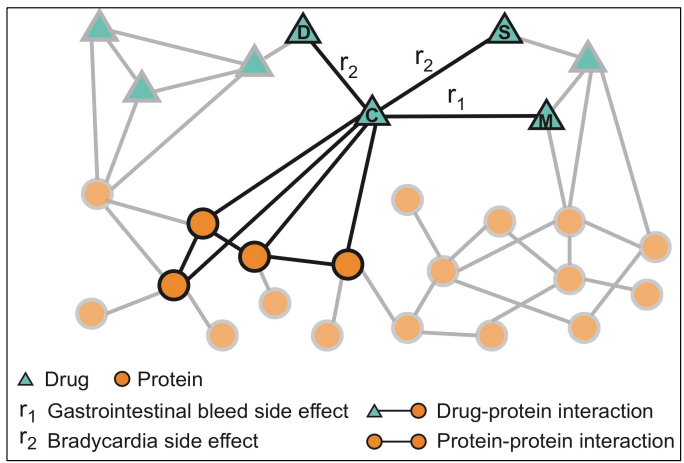
\includegraphics[width = \columnwidth]{figures/GraphNeuralNetworks1/ExampleDrugSideEffects.png}
\end{figure}

\subsubsection{Graph Level Tasks}
\subsubsection*{Examples:}
Road Network as Graph:
\begin{itemize}
    \item \textbf{Nodes:} Road segments
    \item \textbf{Edges:} Connectivity between road segments
    \item \textbf{Prediction:} Time of Arrival (ETA)
\end{itemize}
Embeddings:

Given a graph, find node, edge or graph embeddings.
Node to vector embeddings: Graph Representation Learning

Task: Map Nodes into an embedding space.
Similarity of embeddings between nodes indicate their similarity in the network. For example:
\begin{itemize}
    \item Both nodes are close to each other (connected by an edge)
    \item Encode network information
    \item Potentially used for downstream predictions
\end{itemize}
\begin{figure}[!h]
    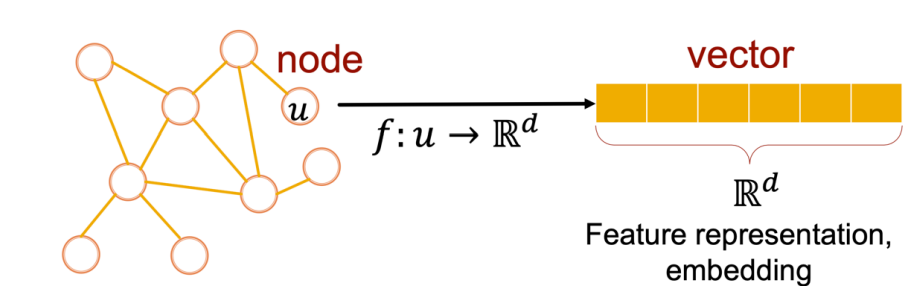
\includegraphics[width = 0.45\columnwidth]{figures/GraphNeuralNetworks1/GraphEmbedding1.png}
    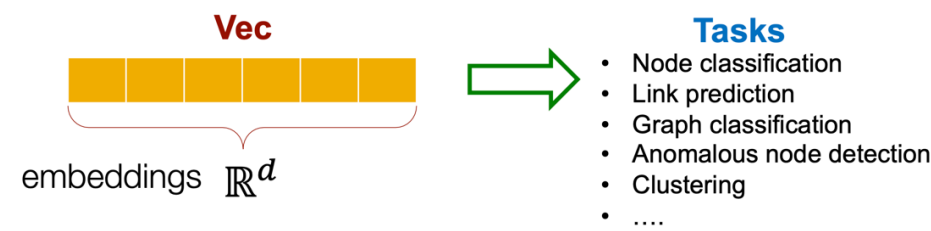
\includegraphics[width = 0.5\columnwidth]{figures/GraphNeuralNetworks1/GraphEmbedding2.png}
\end{figure}

\subsection{Challenges}
How to apply deep learning for these tasks?
Problem with how to use model connectivity!

Adjecency matrices are straight forward but:
\begin{itemize}
    \item Graphs can have millions of nodes
    \item While graphs can also have millions of edges, the matrices would be sparse
    \item Many different adjacency matrices describe the same connectivity
\end{itemize}
\subsubsection{Intuitive method}
Join adjacency matrix and features.
Feed them into deep neural network.
Problems:
\begin{itemize}
    \item Node ordering
    \item Not applicable to graphs of different sizes
    \item Oder of O(|V|) parameters 
\end{itemize}
\subsubsection{Intuitive method:CNNs?}
Generalize convolutions beyond simple lattices (image,text) ?

Graphs can look very different:
\begin{itemize}
    \item No notation of sliding window over graph \dots
    \item Graph is permutation invarant.
\end{itemize}
\subsection{Permutation Invariance and Permutation Equivariance}
Embedding of graph (or nodes) must calculate in the same result regardless of the node ordering.
Consider learning \(f\) that maps a graph \(G = (A,X)\) to a vector.
\subsubsection*{Permutation Invariance}
A graph function is \textbf{permutation invariant} if
\[
f(A,X) = f(PAP^T,PX)
\]
for and permutation \(P\).
\(A\) is the adjacency matrix.
\(X\) is the feature matrix.
\begin{figure}[!h]
    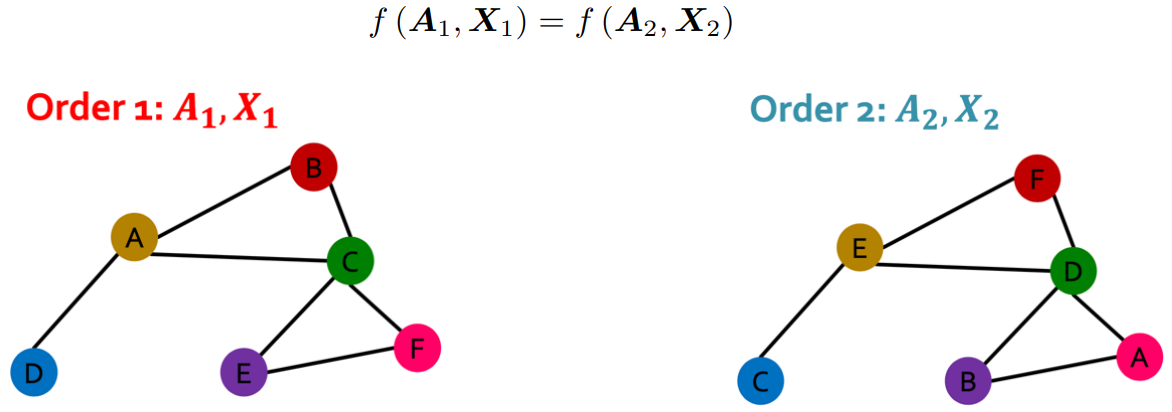
\includegraphics[width = \columnwidth]{figures/GraphNeuralNetworks1/PermutationInvariance.png}
\end{figure}
\subsubsection*{Permutation Equivariance}
A graph function is \textbf{permutation equivariant} if
\[
Pf(A,X) = f(PAP^T,PX)
\]
for and permutation \(P\).
\(A\) is the adjacency matrix.
\(X\) is the feature matrix.
\begin{figure}[!h]
    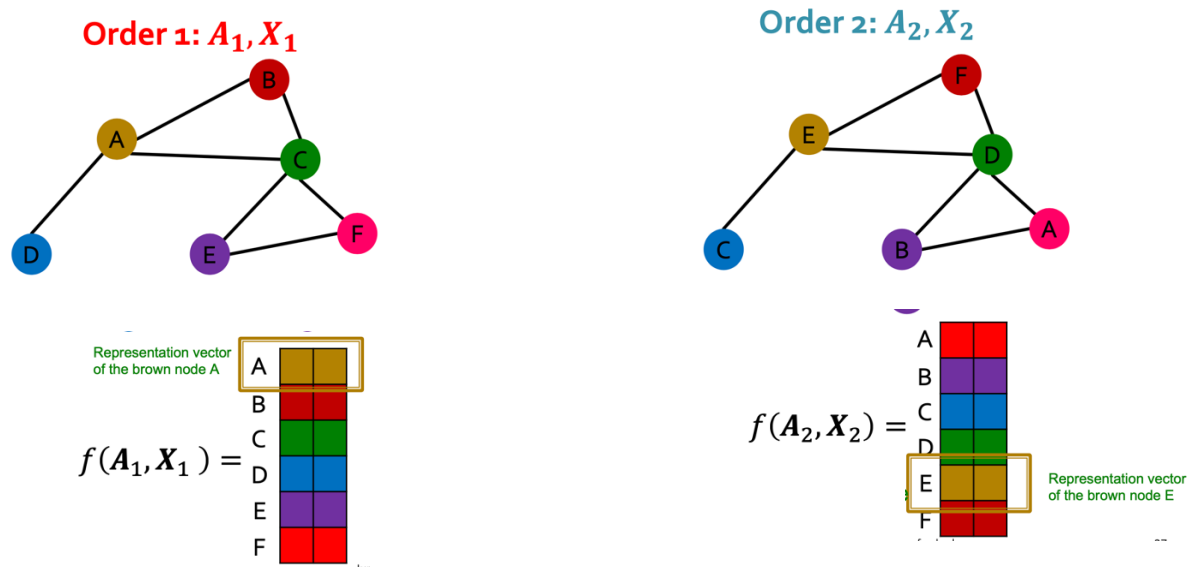
\includegraphics[width = \columnwidth]{figures/GraphNeuralNetworks1/PermutationEquivariance.png}
\end{figure}

\subsection{Representation of sparse matrices}
An \textbf{adjacency list} contains entry of each edge between nodes.
The full graph representation (with features on nodes and edges) can then be described through tensors.
\begin{figure}[!h]
    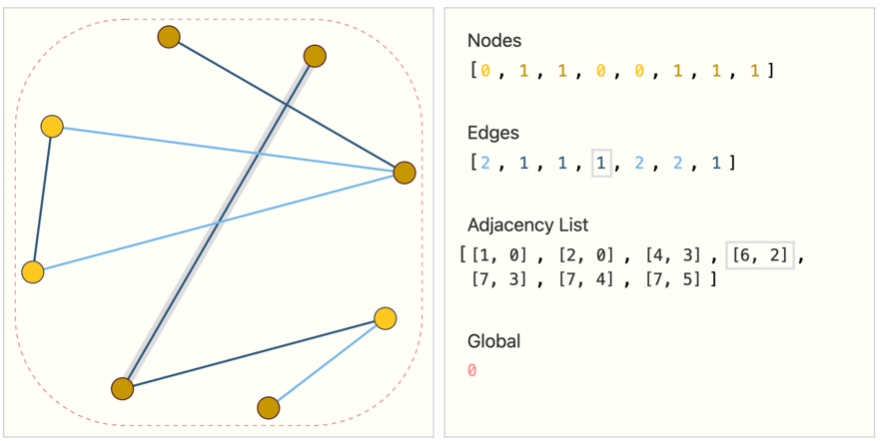
\includegraphics[width = \columnwidth]{figures/GraphNeuralNetworks1/SparseMatrices.png}
\end{figure}

\subsection{Graph Neural Networks (GNN)}
A GNN is an optimizible transformation on all attributes of the graph (nodes, edges, global-context) that preserves graph symmetries (permutation invariance)

Approach to GNNs:
\begin{itemize}
    \item Message passing neural network
    \item Graph net architecture (Graph-In, Graph-Out Model)
\end{itemize}

\subsubsection{GNNs Architecture}
Graph-In, Graph-Out Model:
\begin{itemize}
    \item Input is a graph with information in nodes, edges and global context
    \item These embeddings are continuously transformed without changing the connectivity of the input graph
\end{itemize}

\subsubsection*{A simple GNN}
Use a seperate MLP for each component (node,edge, global context) of the graph.
\begin{figure}[!h]
    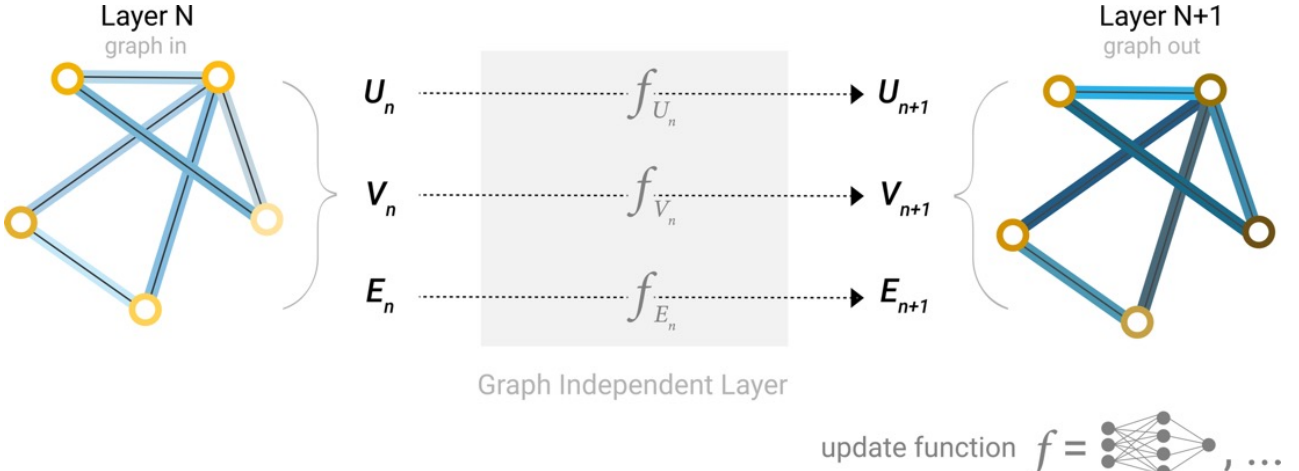
\includegraphics[width = \columnwidth]{figures/GraphNeuralNetworks1/SimpleGNN.png}
\end{figure}

\subsubsection*{Node Predictions}
Add a linear classifier after the last layer for (simple) node prediction.

\begin{figure}[!h]
    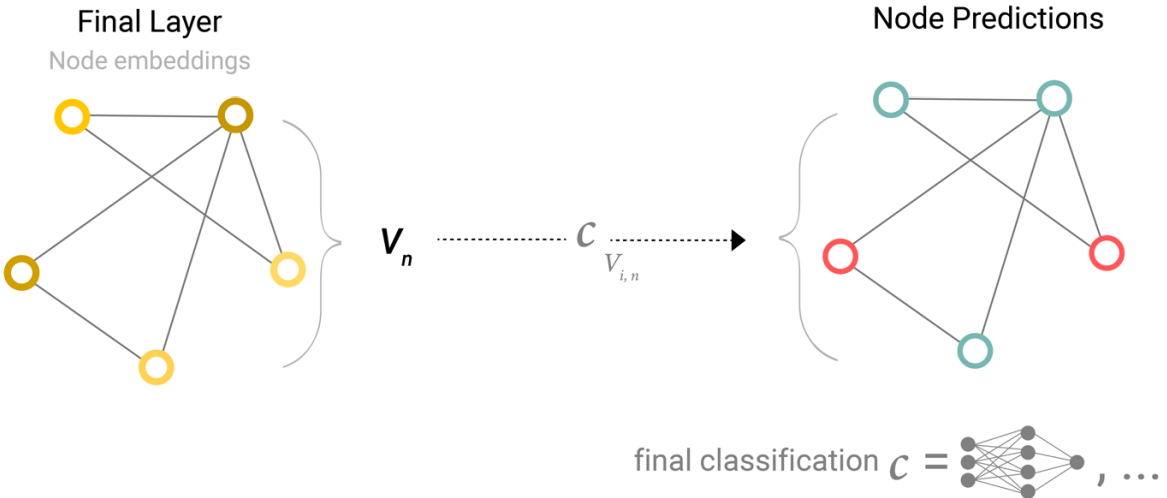
\includegraphics[width = \columnwidth]{figures/GraphNeuralNetworks1/NodePredictions.png}
\end{figure}

\subsubsection*{Node Prediction from edges}
However, we might want to use the information on the edges to make predictions on the nodes.
We can use \textbf{pooling} and \textbf{aggregation}:
\begin{figure}[!h]
    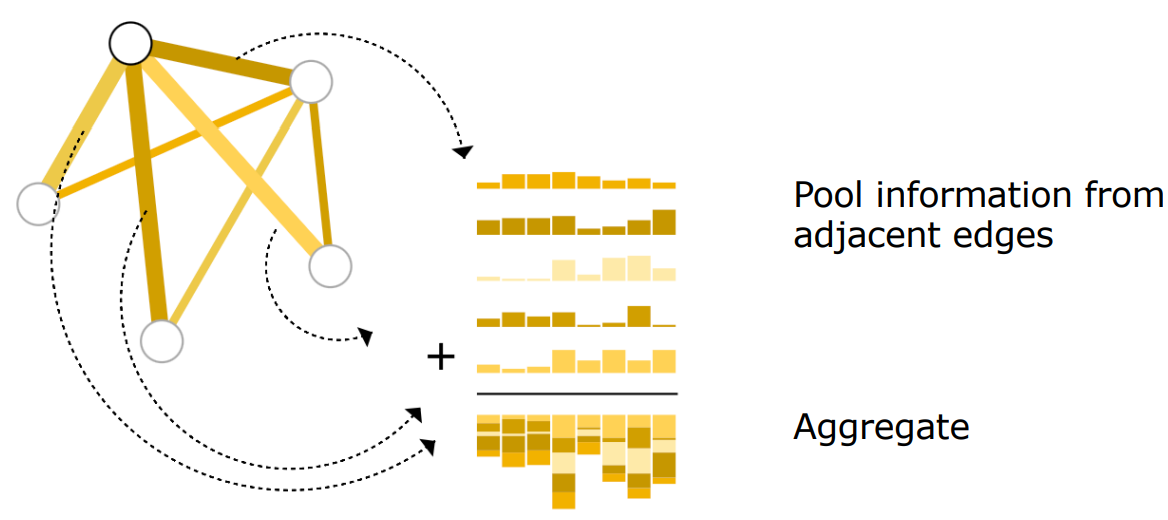
\includegraphics[width = 0.7\columnwidth]{figures/GraphNeuralNetworks1/PredictionFromEdges.png}
\end{figure}

\subsubsection*{Node Prediction from Edges only}
\begin{figure}[!h]
    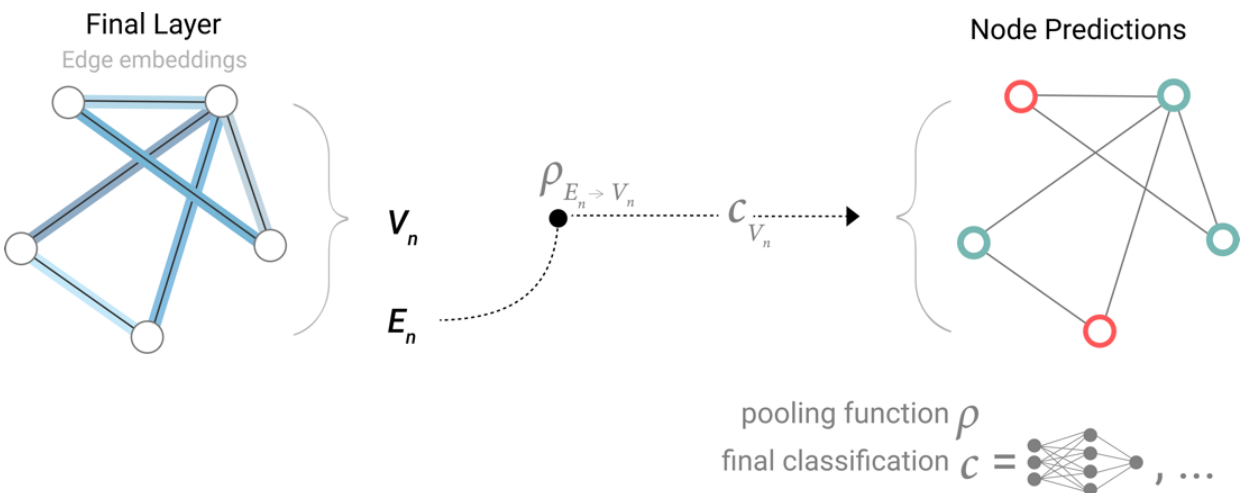
\includegraphics[width = \columnwidth]{figures/GraphNeuralNetworks1/NodePredictionFromEdgesOnly.png}
\end{figure}

\subsubsection*{Edge Prediction from Nodes (only)}
\begin{figure}[!h]
    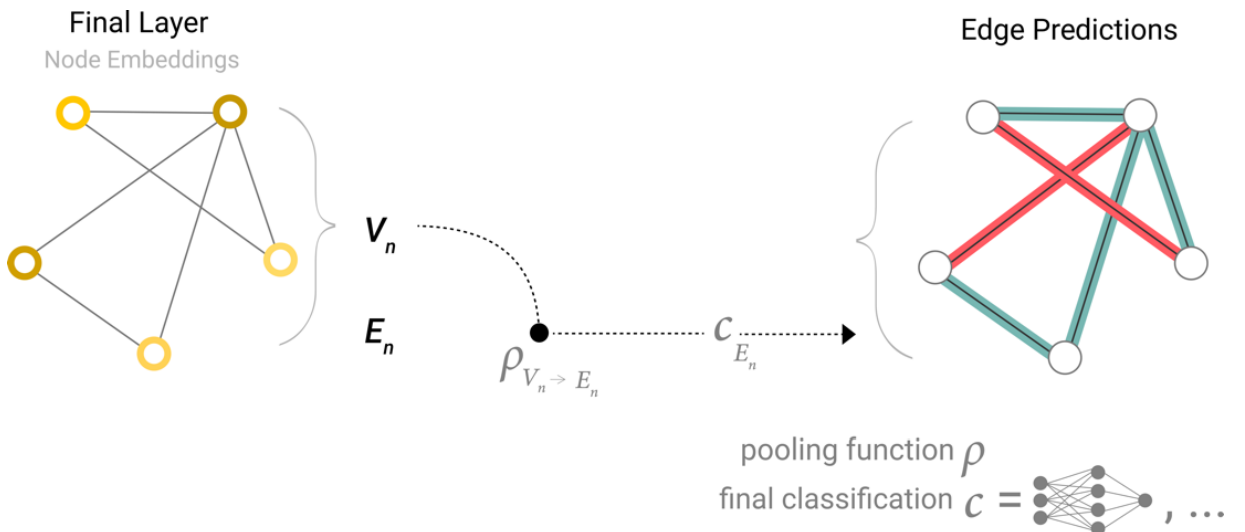
\includegraphics[width = \columnwidth]{figures/GraphNeuralNetworks1/EdgePredictionsFromNodes.png}
\end{figure}

\subsubsection*{Global Prediction}

If we want to make a global prediction, we can pool all node (or edge) information.
This is similar to pooling layers in CNNs.
\begin{figure}[!h]
    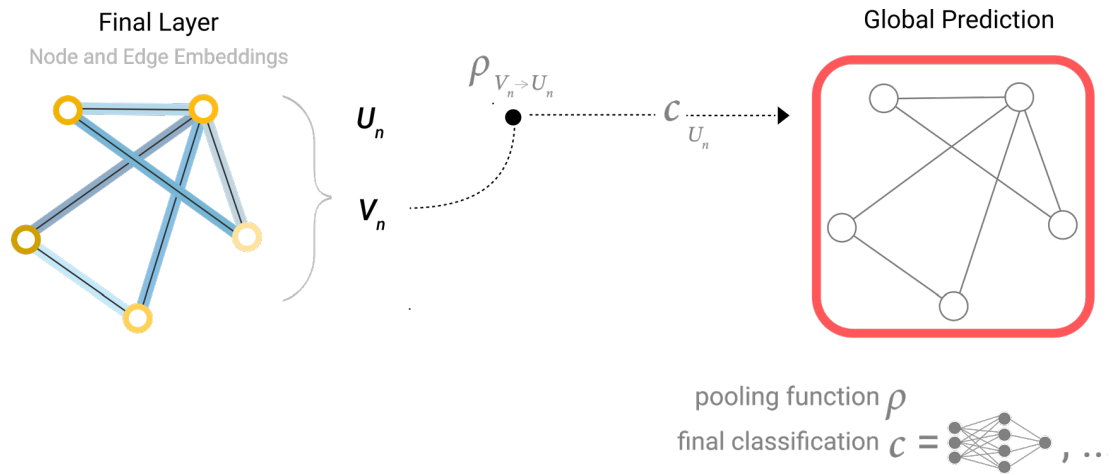
\includegraphics[width = \columnwidth]{figures/GraphNeuralNetworks1/GlobalPrediction.png}
\end{figure}

\subsubsection{Overall simple GNN}
In this simple GNN, connectivity information is only used for pooling, the nodes and edges are processed individually.
\begin{figure}[!h]
    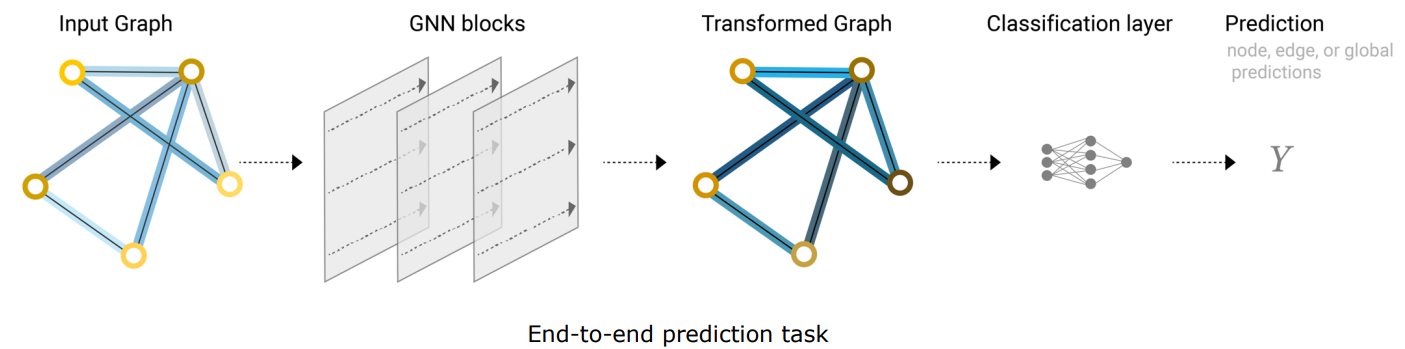
\includegraphics[width = \columnwidth]{figures/GraphNeuralNetworks1/OverallSimpleGNN.png}
\end{figure}

\subsection{Message Passing}
Neighboring nodes (or edges) are now allowed to pass messages, so that our learned embeddings are aware of the graph connectivity.

Message passing:
\begin{itemize}
    \item Gather neighboring node information (embeddings) for each node
    \item Aggregate all messages using aggregate function
    \item Pass the pooled messages through an update function 
\end{itemize}
\begin{figure}[!h]
    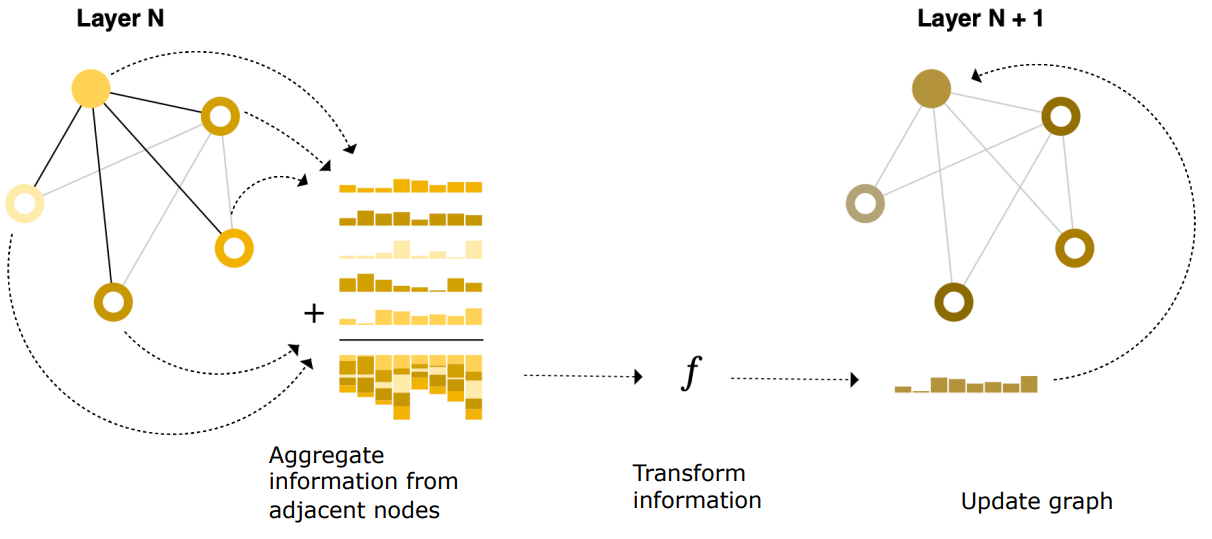
\includegraphics[width = \columnwidth]{figures/GraphNeuralNetworks1/MessagePassing.png}
\end{figure}
\begin{itemize}
    \item Simple GNN operation similar to CNNs, information is updatde with information obtained from neighbors
    \item The number of neighboring nodes can be variable in a graph
    \item The aggregation function must be specified accordingly, for example, sum or averaging are common
    \item By stacking message passing, a node can incorporate information from nodes further away
\end{itemize}
\subsubsection{Simple Message Passing}
\begin{figure}[!h]
    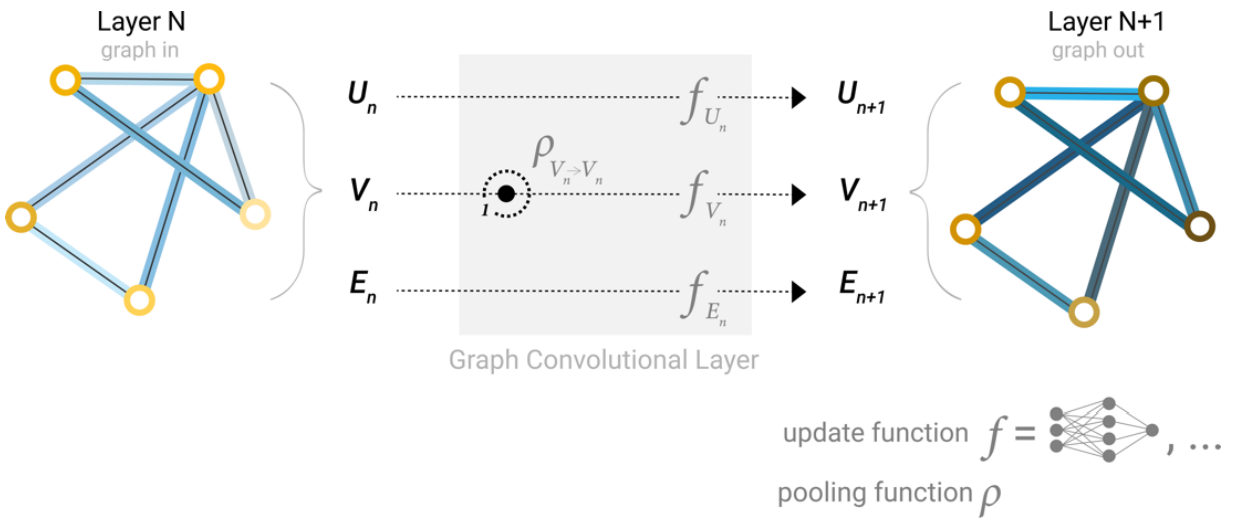
\includegraphics[width = \columnwidth]{figures/GraphNeuralNetworks1/SimpleMessagePassing.png}
\end{figure}
	\section{Graph Neural Networks 2}
\subsection{Homogenous Graphs}
\(G = (V,E,)\)
\begin{table}[!h]
    \begin{tabular}{lr}
    Nodes     &  \(v_i \in V\)\\
    Edges      &  \((v_i,r,v_j) \in E\)
    \end{tabular}
\end{table}
Nodes and edges can have \textbf{attributes / features}.
Directed or undirected edges.

\subsection{Graphs}
Connectivity is specified by the \textbf{adjacency} matrix \textbf{A}.
\textbf{A} is often stored in a \textbf{sparse} formate.

\begin{figure}[!h]
    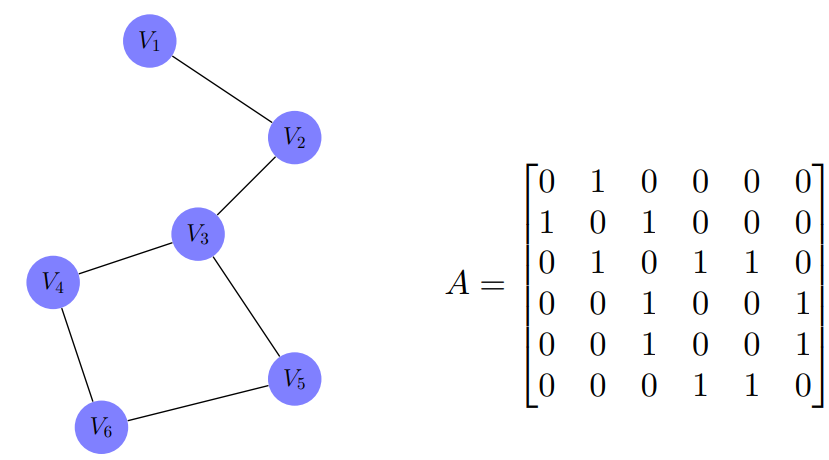
\includegraphics[width = \columnwidth]{figures/GraphNeuralNetworks2/SparseFormat.png}
\end{figure}

\subsection{Features}
Each node can contain a feature vector
\(x_i\) and each edge a feature vector \(e_{ij}\).
There might also be a global feature vector \(U\).

Many GNN approaches only use node features, so the graph is defined by \((A,X)\).
\begin{figure}[!h]
    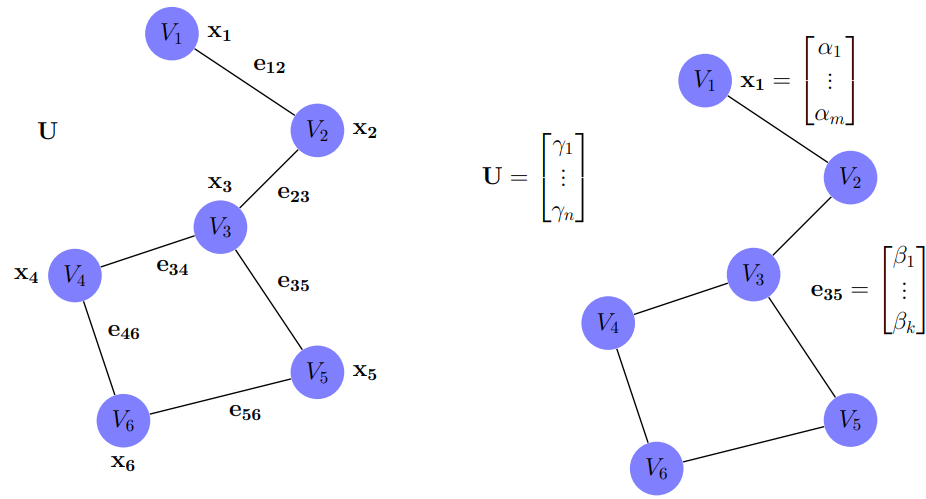
\includegraphics[width = \columnwidth]{figures/GraphNeuralNetworks2/Features.png}
\end{figure}

\subsection{GNNs: Idea}
Each layer of a GNN will \textbf{transform} the \textbf{transform} of the nodes and edges.
This is similar to an image going through the layers of a CNN.
\begin{figure}[!h]
    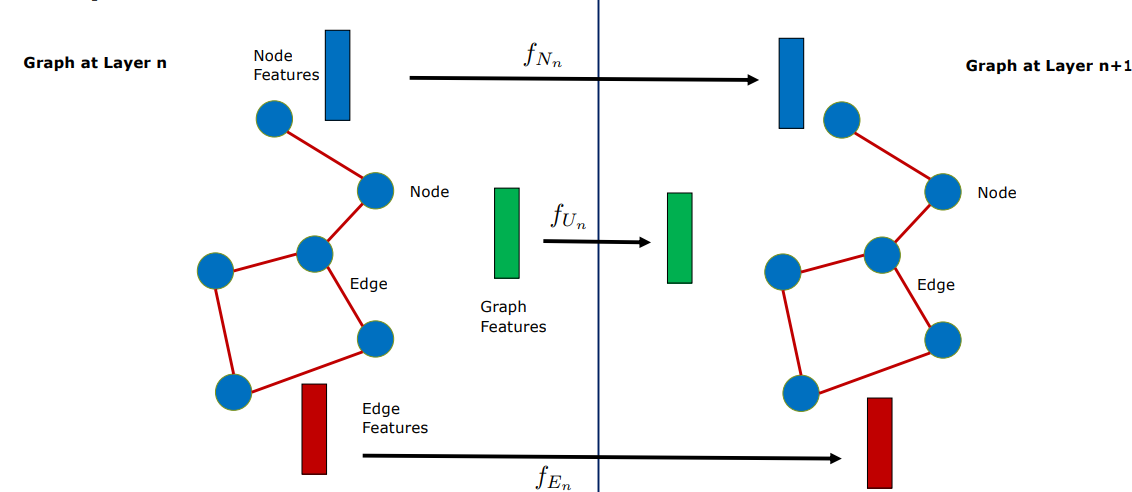
\includegraphics[width = \columnwidth]{figures/GraphNeuralNetworks2/GNNsIdea.png}
\end{figure}
\subsubsection{Feature Transformation}
\begin{itemize}
    \item The intermediate feature values for the nodes are commonly indicated by \(\mathbf{h}\) (similar to the hidden states in RNNs) and the output of the transformation is \(\mathbf{z}\).
    \item The dimension of the hidden values might change (similar to channels in CNNs).
\end{itemize}
\[
\mathbf{x} = 
\begin{bmatrix}
\dots \\
\dots \\
\dots
\end{bmatrix}
\longrightarrow
\mathbf{h}_1 = 
\begin{bmatrix}
\dots \\
\dots \\
\dots 
\end{bmatrix}
\longrightarrow
\hdots
\longrightarrow
\mathbf{h}_n = \mathbf{z} = 
\begin{bmatrix}
\dots \\
\dots \\
\dots
\end{bmatrix}
\]

\subsection{Graph Convolutions by Spectral Methods}
Convolutions turn into element-wise multiplications in the spectral domain by the Fourier Transform.
After the convolutions, the signal can be turned back using the inverse Fourier Transform.

The Graph Fourier Transform can be calculated using the Eigenvalues of the Laplacian:
\[
L = U\Lambda U^T \qquad \Lambda = \text{diag}(\left[\lambda_0,\lambda_1,\dots,\lambda_n\right])
\]
Convolution with learnable function g:
\[
g \ast x = F^{-1}(F(g)\times F(x)) = U(U^Tg\times U^Tx)
\]
\subsection{Some graph math for calculating GNNs}
\begin{itemize}
    \item The \textbf{degree} of a node is the number of its direct neighbours.
    \item If \(mathbf{A}\) is given, the degree can be calculated by summing the nodes
    \item It is usually written as a diagonal matrix \(mathbf{D}\)
\end{itemize}
\begin{figure}[!h]
    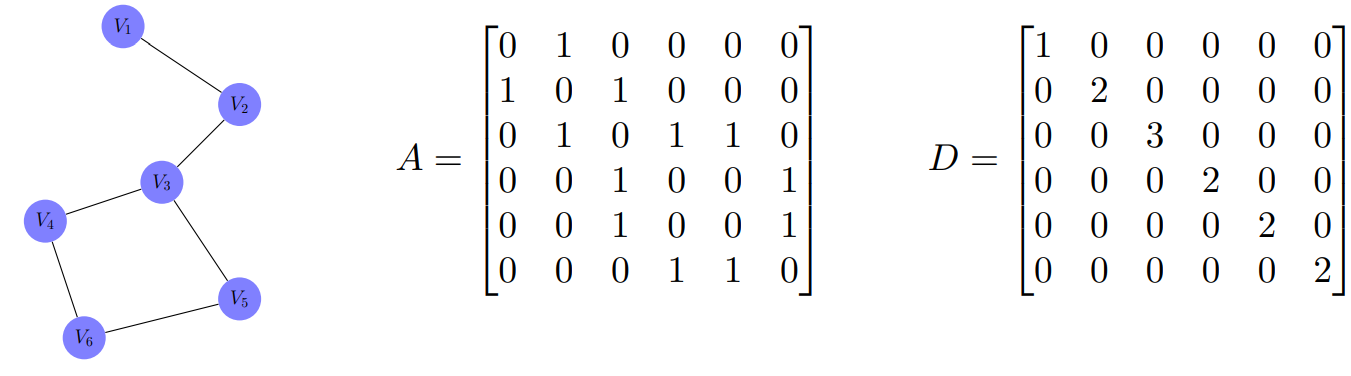
\includegraphics[width = \columnwidth]{figures/GraphNeuralNetworks2/MathForGNNS.png}
\end{figure}

\subsubsection{Graph Laplacian}
\begin{table}[!h]
    \begin{tabular}{lr}
    Graph Laplacian    &  \(L = D - A\)\\
    Edges with relation types     &  \(L = 
    \begin{bmatrix}
      1  & -1 &  0 &  0 &  0 &  0 \\
     -1  &  2 & -1 &  0 &  0 &  0 \\
      0  & -1 &  3 & -1 & -1 &  0 \\
      0  &  0 & -1 &  2 &  0 & -1 \\
      0  &  0 & -1 &  0 &  2 & -1 \\
      0  &  0 &  0 & -1 & -1 &  2 \\
    \end{bmatrix}\)\\
    Normalized Laplacian    & \(L = I-D^{-\frac{1}{2}}AD^{-\frac{1}{2}}\)
    \end{tabular}
\end{table}
\subsubsection{Spectral Methods}
\begin{itemize}
    \item The filter in spectral networks is applied over the entire (connected) graph, so there is no locality
    \item Caculation of the eigenvalues is inefficient
    \item ChebNets use Chebyshew Polynomials to define a convolution that uses only a k-hop neghborhood of a node
    \item Graph Convolutional Networks (GCN) use \(k = 1\)
\end{itemize}
\subsection{Graph Convolutional Networks (GCN)}
\begin{itemize}
    \item Enforce self-connection by using\[
    \tilde{A} = A + I_n \qquad \tilde{D}_{ij} = \sum_{j}^{}\tilde{A}_{ij}
    \]
    \item and calculate the normalized Laplacian, which now has eigenvalues in \([0 \dots 1]\) (no exploding gradients)
    \[
    L_{norm} = \tilde{D}^{-\frac{1}{2}}\tilde{A}\tilde{D}^{-\frac{1}{2}}
    \]
    \item The update rule then becomes:
    \[
    H^{l+1} = \sigma(\tilde{D}^{-\frac{1}{2}}\tilde{A}\tilde{D}^{-\frac{1}{2}}H^{(l)}W^{(l)})
    \]
\end{itemize}
The update rule can be written in the spatial domain as 
\[
h_i^{(l)} = \sigma\left(\sum_{i \in N_j}c_{ij}Wh-j\right)
\]
where
\[
c{ij} = \frac{1}{\sqrt{|N_i||N_j|}}
\]
and \(|N_i||N_j|\) are the sizes of the node neighborhood.
\begin{figure}[!h]
    \centering
    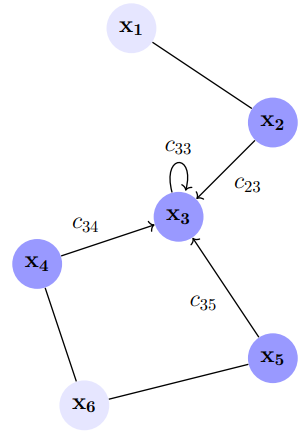
\includegraphics[width = 0.3\columnwidth]{figures/GraphNeuralNetworks2/GCN.png}
\end{figure}
\subsubsection{Node Classification}
\begin{itemize}
    \item For node classification, a classifier can be added that uses the output \(\mathbf{z}\) of a node for classification.
    \item Node classification can be \textbf{semi-supevised}: The GNN is trained on the graph which contains some labelled node and then used to predict the classes of the remaining nodes.
\end{itemize}
\subsubsection{Graph Convolutional Networks: Loss}
Loss for semi-supervised learning (node classification) in the spectral formulation
\[
    \mathcal{L} = \mathcal{L}_0 + \lambda \mathcal{L}_{reg} \quad \mathcal{L}_{reg} = \sum_{i,j}A_{ij}||f(X_i)- f(X_j)||^2 = f(X)^T\nabla f(x)
\]
\(\mathcal{L}_0\) is the supervised loss with respect to the labelled parts of the graph, \(X\) are the node features and \(f\) a Neural Network.

\subsection{Semi-supervised node classification with GCN: Example}
\subsubsection{Node Embeddings}
\begin{itemize}
    \item Node embeddings map a node to a feature vector \(z\)
    \item Similarity in the embedding space should approximate similarity in the graph
    \item This is an \textbf{unsupervised} task
\end{itemize}
\subsubsection*{Node Embeddings: Variational Graph Auto Encoder (VGAE)}
Use a Variational Auto Encoder (VAE) to encode and decode a graph:
\begin{itemize}
    \item The encoder calculates an embedding or \textbf{latent variable z}
    \item The decoder calculates the graph from z by predicting the \textbf{adjacency matrix A}
\end{itemize}
For a simple auto encoder, this can be achieved by
\[
\hat{\mathbf{A}} = \sigma(\mathbf{Z}\mathbf{Z}^T), \text{with} \mathbf{Z} = GCN(\mathbf{X},\mathbf{A})
\]
I.e. the encoder is a graph convolutional network, the decoder a simple inner product.
\begin{itemize}
    \item (Variational Auto Encoder use a more complicated loss function to ensure z is Gaussian distributed)
    \item VGA can be used for \textbf{link prediction}
\end{itemize}

\subsubsection{Spacial Methods}
Spetial methods define convolutions directly on the graph, based on the topology.
Usually:
\begin{itemize}
    \item The features vectors are transformed
    \item They are aggregated in a permutation-invariant function
    \item The feature vector of each node is updated from its current value and the aggregated neighborhood representation
\end{itemize}
Popular methods:
\begin{itemize}
    \item GraphSAGE
    \item Message Passing Neural Network (MPNN) 
\end{itemize}
\subsubsection*{GraphSAGE}
Update node features as
\[
\mathbf{x}_i' = \mathbf{W}_1\mathbf{x}_i + \mathbf{W}_2 \times \text{mean}_{j \in \mathcal{N}(i)}\mathbf{x}_j
\]

with (optionally) first projecting \(x_j\)
\[
\mathbf{x}_j \leftarrow \sigma (\mathbf{W}_3 \mathbf{x}_j + \mathbf{b})
\]
For training on a number of input nodes (for a minibatch), their neighborhood is sampled as needed for computation.
\begin{figure}[!h]
    \centering
    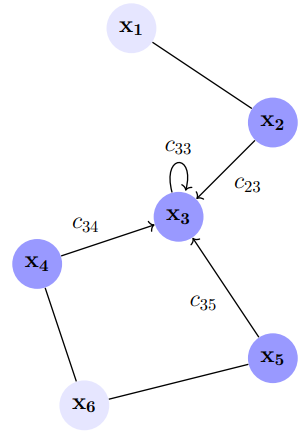
\includegraphics[width = 0.3\columnwidth]{figures/GraphNeuralNetworks2/GCN.png}
\end{figure}
Possible aggregation functions are:
\begin{itemize}
    \item Mean:
    \[
        \mathbf{h}_v^k \leftarrow (\mathbf{W} \cdot \text{MEAN}(\left\{\mathbf{h}_v^{k-1}\right\}\cup\left\{\mathbf{h}_u^{k-1},\forall u \in \mathcal{N}(v)\right\}))
    \]
    \item LSTM: LSTM cell with random permutation of node's neighbors
    \item Pooling:
    \[
        \text{AGGREGATE}_k^{pool} = \max\left(\left\{\sigma(\mathbf{W}_{pool}\mathbf{h}_{ui}^k + \mathbf{b}),\forall u_i \in \mathcal{N}(v)\right\}\right)
    \]
    \item Experiments show that LSTM and pooling perform best.
\end{itemize}


\subsection{Message Passing Neural Networks (MPNN)}
\begin{itemize}
    \item Message \(m_{ij}\) can be sent across edges between nodes \(V_i\) and \(V_j\) and are computed using a message function (small MLP).
    \[
    m_{ij} = f_e(h_i,h_j,e_{ij})
    \]
    \item Messages are aggregated using a permutation-invariant function (sum, mean, max, etc.)
    \item The aggregated message is combined with the current node features and updated using another function
    \[
    h_i = f_v(h_i,\sum_{j \in N_i}m_{ji})
    \]
\end{itemize}
\begin{figure}[!h]
    \centering
    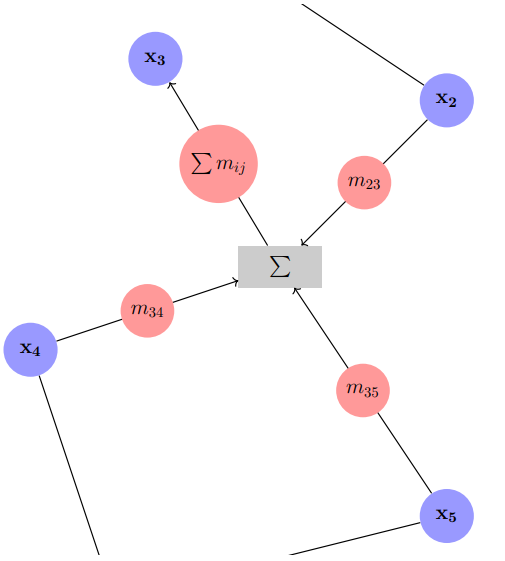
\includegraphics[width = 0.3\columnwidth]{figures/GraphNeuralNetworks2/MessagePassing1.png}
    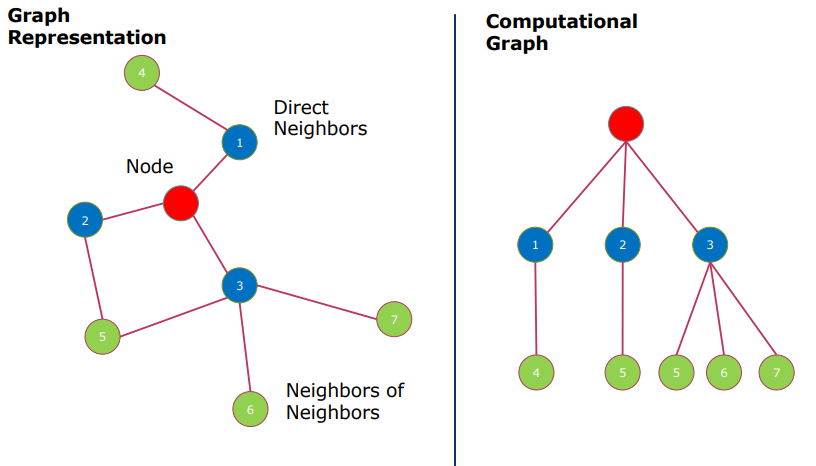
\includegraphics[width = 0.65\columnwidth]{figures/GraphNeuralNetworks2/MessagePassing2.png}
\end{figure}

\subsection{Graph Attention Networks}
In GCNs features from neighboring nodes are weighted by their degree
\[
h_i^{(i)} = \sigma \left(\sum_{i \in N_j}\frac{1}{\sqrt{|N_i||N_j|}}Wh_j\right)
\]
these are statistically defined from the graph and might not always be beneficial.
\begin{itemize}
    \item Simple, spatial convolutions can also be calculated without these weights, or
    \item The weights could be calculated from the features to see which nodes are more important
    \item Calculate attention scores on a trainable linear transform of the node featues for the nodes \(j \in \mathcal{N}_i\) neighbors:
    \[
    e_{ij} = a(\mathbf{Wh}_i,\mathbf{Wh}_j)\\
    \alpha_{ij} = softmax_j(e_{ij}) = \frac{\text{exp}(e_{ij})}{\sum_{k\in\mathcal{N}_i}\text{exp}(e_{ik})}
    \]
     \item The attention mechanism here is a single layer MLP (instead of the scalar dot product)
\end{itemize} 
The new features of a node are then calculated as 
\[
\vec{h}_i' = \sigma \left(\sum_{j \in \mathcal{N}_i} \alpha_{ij}\mathbf{W}\vec{h}_j\right)
\]
additionally Multi-headed Attetion is used
\begin{figure}[h!]
    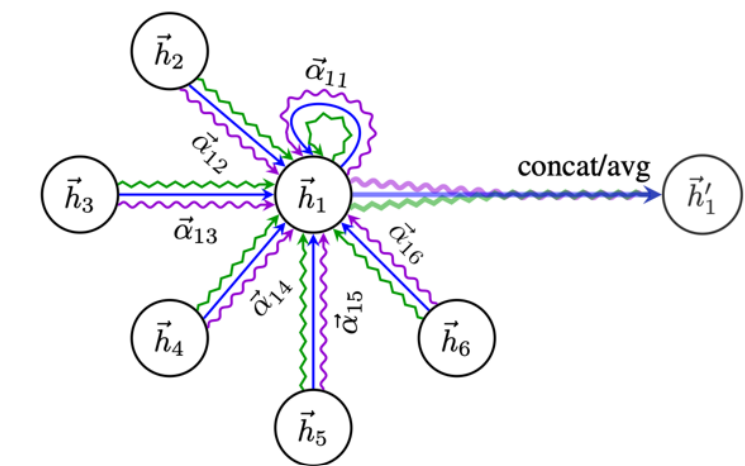
\includegraphics[width = 0.5\columnwidth]{figures/GraphNeuralNetworks2/GraphAttentionNetworks.png}
\end{figure}

\subsection{Graph Classification}
\begin{itemize}
    \item For graph classification, often the resulting output features \(\mathbf{z}\) of the nodes are used and combined in a so-called \textbf{readout} operation
    \item This results in a single vector for the graph, which is then used as input for classification
    \item Graph Classification is usually \textbf{supervised learning}, the GNN is trained on many different graphs, and then applied to a new graph
\end{itemize}

\subsection{Conclusion}
\begin{itemize}
    \item GNNs are an evolving and active field
    \item There are many different approaches and no cnosensus yet
    \item Some approaches are coupled with their applications (node/graph level tasks \& unsupervised, semi-supervised and supervised settings)
    \item Message passing provides a conveniant way to describe many variants of GNNs
\end{itemize}
	\section{Explainable AI 1}
What makes XAI difficult?:
\begin{enumerate}
    \item \textbf{The missingness problem:}
    
    How to properly define missingness
    \item \textbf{The correlation problem}
    
    How to tractably consider feature dependence
\end{enumerate}

\subsection{Nomenclature}
\begin{itemize}
    \item \textbf{Global:} Creating a summary of which features most influence predictions across all instances in a dataset, such as using SHAP to determine overall feature importance in a model
    \item \textbf{Surrogat:} Using a decision tree to approximate and explain a complex neural network model's behaviour by replicating its predictions
    \item \textbf{Attributions:} A heatmap that shows which pixel in an image contributed the most to a model's decision that the image contained a dog
    \item \textbf{Intrinsic:} A simple decision tree model used for classification where the splits and rules can be directly interpreted by humans
    \item \textbf{Local:} Analyzing why a specific instance of a loan application was approved or denied by examining factors unique to that case
    \item \textbf{Counterfactual:} Suggesting that if a loan applicant's income had been 5000\$ higher, thier loan would have been approved
    \item \textbf{Post hoc:} Using an XAI method explain predictions of a black-box model after the model has made a prediction
\end{itemize}

\subsection{Grad-CAM}
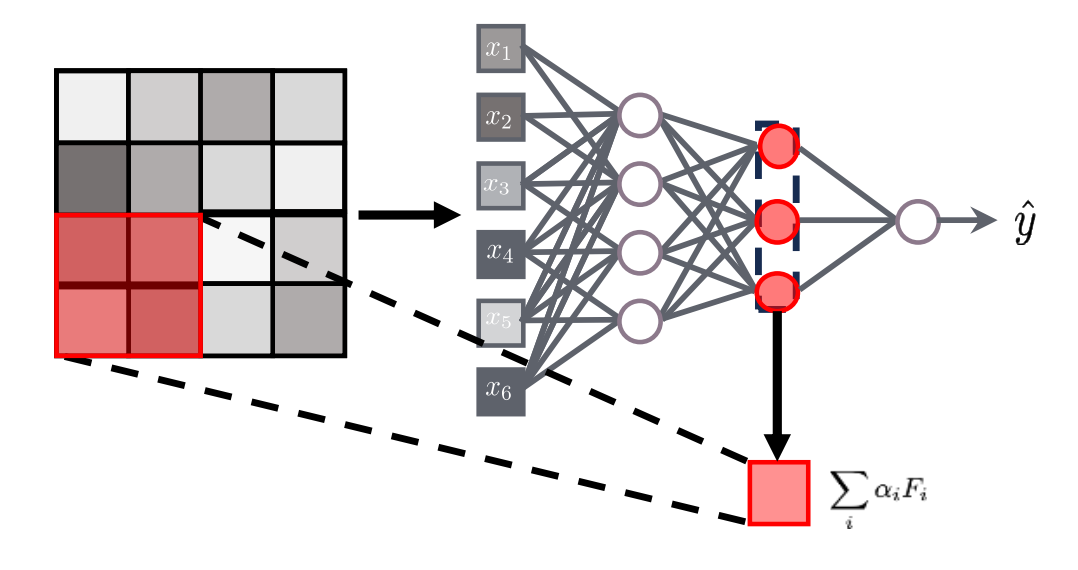
\includegraphics[width = \columnwidth]{figures/XAI1/GradCAM.png}

\subsection{interpreable}
\begin{itemize}
    \item These are simple models that we call white box models
    \item They require no fanccy XAI methods to interpret
    \item They are boring and make to many assumptions about the data
    \item They often from a vital component of some extravagant, powerful XAI methods, see LIME, Grad-CAM, SHAP, etc.
\end{itemize}
\subsection{Linear models}
\begin{figure}
    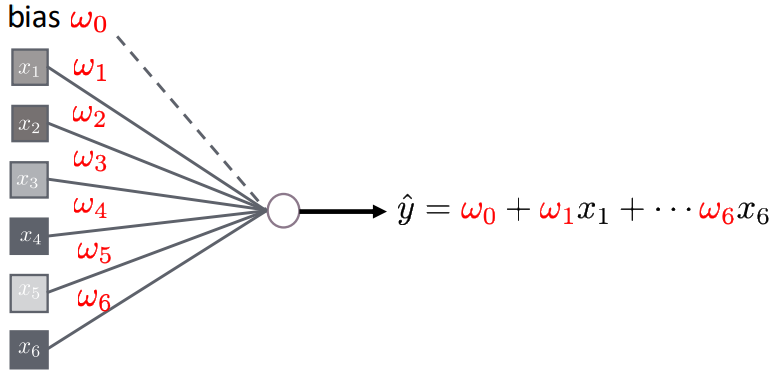
\includegraphics[width = 0.8\columnwidth]{figures/XAI1/LinearModels.png}
\end{figure}
Find optimal weights by minimizing MSE
\[
w^* = arg \min_{w_0 + \dots w_p}\sum_{i = 1}^{n}\left[y^{(i)}-\left(\mathbf{w}_0 + \sum_{j = 1}^{p}\mathbf{w}_j\mathbf{x}_j^{(i)}\right)\right]^2
\]

Interpretable metrics:
\begin{enumerate}
    \item Weights: The magnitude of a weight is proportional to the importance
    \item \(\text{R}^2\): Are the weights worth interpreting? i.e., is our model good?
    \item Adjusted \(\text{R}^2\): Improved to remove artifically inflating the fit by adding more features
\end{enumerate}
\subsubsection{Weights}
\begin{itemize}
    \item \(w = 0\):Weight of zero  means feature is unimportant because no matter the value of x, it gives the same result.
    \item \(w = 1\): Weight is larger, the y-value depends on the x-value. Negelcting the feature dependence will result in large errors
\end{itemize}
\subsubsection{\(\text{R}^2\)}
\begin{itemize}
    \item \(SEE\): Variance after the model has been fitted
    \item \(SST\): Natural amount of variance within the data
\end{itemize}
Exaplaining Variance with \(R^2 = 1 - SSE /SST\).
\[
SSE = \sum_{i = 1}^{n}\left(y^{(i)}-\hat{y}^{(i)}\right)^2 \qquad SST = \sum_{i = 1}^{n}\left(y^{(i)}-\overline{y}^{(i)}\right)^2
\]
\begin{itemize}
    \item \(R^2 = 1\): SST non-zero, SSE zero (perfect fit), weight are meaningfull
    \item \(R^2 < 1\): SST larger, SSE non-zero, weight are meaningfull
    \item \(R^2 \rightarrow 0\): Even though weight is large, the interpretability should not be trusted because the model does not capture the variance of the data. SEE and SST become comperable.
    \item \(R^2 < 0\): SEE bgger than SST,negative number, adverse model. Normally the fit would lie in the middle and thus result in smaller variance than the natural data variance
\end{itemize}
\subsubsection{Adjusted \(R^2\)}
Fix using the adjusted \(R^2\) metric:
\[
\overline{R}^2  = 1-(1-R^2)\frac{n-1}{n-p-1}
\]
p = \# of features, n = \# of instances.
Adjusted \(R^2\) penalizes for model complexity.

\subsubsection*{What happens if we have thousands of features}
\begin{itemize}
    \item Interpretability decreases
    \item Might even have more features than instances
\end{itemize}
Lasso regularization to introduce sparsity via the L1-norm.
\[
\mathcal{L} = \frac{1}{n}\sum_{i =1}^{n }\left(y^{(i)} - x_i^T\mathbf{w}\right)^2 + \lambda ||\mathbf{w}||_1
\]
Model not only wants to predict the data, but also wants to make the weights small.

\subsection{Decision-Trees}
Goal is to have good purity and loq complexity so tree model generalizes.

The idea of entropy can be used to achieve leaf purity
\[
H(D) = -\sum_{i = 1}^{k}p(C_i) \cdot log_2(p(C_i))
\]
\(C_i = \)black and white balls (2 classes)
\subsubsection{Grow a tree}
\begin{enumerate}
    \item For all possible features and splits calculate H
    \item Calculate weighted entropy for each split (larger purer states better)
    \[
    H_{after split} = \frac{|D_1|}{|D|}H(D_1) + \frac{|D_2|}{|D|}H(D_2)
    \]
    \item Calculate information gained from each split
    \[
    IG(D,A) = H(D) - H_{after split}
    \]
    \item Choose the feature and split with the highest information gain
\end{enumerate}
Reapeat until subsets are all pure, tree reaches max depth, minimum number of samples is reached.
\subsubsection{Feature importance}
\begin{itemize}
    \item \textbf{Feature split depth}: Features that are used higher up in the tree are more important
    \item \textbf{Feature split frequanzy}:
    Features that are used more often are more important
\end{itemize}
\subsubsection{Decision Trees XAI}
\begin{enumerate}
    \item \textbf{Feature importance} based on sum of information gain (Gini impurity)
    \item \textbf{Rule Extraction} for instance-level, intuitive explanations
    \item \textbf{Leaf Node Analysis}, look at distribution of features in a singel leaf
    \item \textbf{Counterfactual Explanations}, closest path resulting in different classification
\end{enumerate}
\subsubsection{Summary Decision Tree}
\begin{itemize}
    \item Trees are built using the idea of entropy
    \item The objectiv is to have leaf purity i.e., low entropy
    \item Features and splits are determined by maximizing information gain, this is the recipe to lower tree entropy
    \item Overfitting is prevented by hardcoding max tree depth, leaf purity threshold, etc.
    \item XAI local explanation by studying statistics of each group, counterfactuals by finding closest path that result in calss flips, rule based explanations for short trees, sum of weighted information gain for feature ranking
    \item Greedy or deterministic
\end{itemize}
\subsubsection{Summary Random forests}
\begin{itemize}
    \item Can be used for computationally cheap high performance outlier detection
    \item Is comparable to more complex methods such as single-class SVM and Gaussian mixture models
    \item Uses forests and random numbers
    \item Randomly select feature, randomly select split value
    \item Outliers are isolated in leaf nodes closer to the roots
    \item Aggregate results of isolating leaf depth is used to stabalize the random number
    \item Random numbers power the idea, and aggregates of many trees (forests) stabilize the results
\end{itemize}

\subsection{Plot based methods}
\subsubsection{Partial Dependency Plot (PDP)}
First order approximation of feature dependence. Assume features are uncorrelated

Procedure (Linearly):
\begin{enumerate}
    \item Select feature index to analyte (i = 2)
    \item Find unique values for this feature
    \item Order values of this features in ascending order
    \item Set feature \(i_0\) for all instances and calculate average
    \item Repeated this for \(i_1\) to \(i_n\) tracing out a curve
\end{enumerate}
Vectorize by replacing entire column with single featured value.
Problems: Examples might not be physical because features are most likely not independent.
\subsubsection{Individual Conditional Expectaion Plot (ICE)}
Second order approximation of feature dependency

Procedure (Linearly):
\begin{enumerate}
    \item Select feature index to analyte (i = 2)
    \item Find unique values for this feature
    \item Order values of this feature in ascending order
    \item Take single instance ans calculate BB-model output varying feature \(i\) over all its values to trace out a curve
    \item Reapeated for sub subsets
\end{enumerate}
\subsubsection{Summary}
\begin{itemize}
    \item Easy intuitive way to interpret a models dependency on a feature
    \item PDPs might hide critical information
    \item ICE shows more detail but are computationally expensive to calculate and can get visually overwhelming
    \item Both suffer from sparse data
    \item Both assume that features are independent, this might result in the generation of unrealistic data instance
\end{itemize}
	% \input{Sections/04_Interprozesskommunikation}
	% \input{Sections/06_Deadlocks_PriorityInversion}
	% \input{Sections/07_Scheduling}
	% \input{Sections/08_Speicherhierarchie}
	% \input{Sections/10_Speicherverwaltung}
	
	% \input{Sections/99_CodeBeispiele}

\end{document}
